%% STRUCTURED CUSTOMIZATION OF ARSCLASSICA / CLASSIC THESIS TEMPLATE
%% ---------------------------------------------------------------------------


%% --- GLOBAL BASIC LAYOUT ---------------------------------------------------
\documentclass[a4,dottedtoc]{scrbook}
\usepackage[top=3cm,bottom=3cm,left=3cm,right=3cm]{geometry} % Managing custom margins
\usepackage{changepage} 
                        % Commands to change the page layout in the middle of a document, and to robustly check for typesetting on odd or even pages
\usepackage{setspace}   %Needed for \onehalfspacing
\usepackage{calc} 
                        % To perform arithmetic on the arguments of the LATEX commands \setcounter, \addtocounter, \setlength, and \addtolength [USED SILENTLY!]
%% ---------------------------------------------------------------------------


%% --- FONTS & ENCODING ------------------------------------------------------
\usepackage[american, italian]{babel}
\usepackage[utf8]{inputenc}          % Unicode standard UTF-8
\usepackage[T1]{fontenc}             % Output font encoding
\usepackage{amsmath,amssymb,amsthm}
%% ---------------------------------------------------------------------------


%% --- REFERENCES & BIBLIOGRAPHY ---------------------------------------------
\usepackage{varioref} % \vref and \vpageref ('decorated' references...)
\PassOptionsToPackage{
        natbib=true,
        style=numeric,
        citestyle=numeric-comp,
        sorting=nyvt, % name,year,volume,title
        maxnames=3,
        minnames=1,
        hyperref=true,
        backend=biber,
        parentracker=true,
        url=false,
        doi=false,
        isbn=false,
        eprint=false,
        backref=true,
            }   {biblatex}
\usepackage{biblatex}
\addbibresource{Bibliografia/articoli.bib}
\addbibresource{Bibliografia/testi.bib}
\addbibresource{Bibliografia/web.bib}
\usepackage[autostyle]{csquotes}          
                                    % Ensures that quoted texts are typeset according to the rules of your main language. (>babel)
%% ---------------------------------------------------------------------------


%% --- FIGURE MAGIC ----------------------------------------------------------
\usepackage{subfig}
\usepackage{caption}
\usepackage{graphicx}
\usepackage{xcolor}
% MAYBE ADD XCOLOR AND DEFINE THE UNITS OFFICIAL PANTONE
%% ---------------------------------------------------------------------------


%% --- HYPERLINKS & METADATA -------------------------------------------------
\usepackage{hyperref}
\hypersetup
{
	%bookmarks=true,         % show bookmarks bar
	unicode=true,           % non-Latin characters in Acrobat’s bookmarks
	pdftoolbar=false,       % show Acrobat’s toolbar?
	pdfmenubar=true,        % show Acrobat’s menu?
	pdffitwindow=false,     % window fit to page when opened
	pdfstartview={FitH},    % fits the width of the page to the window
	pdfauthor={Anaïs Trinca},
	pdftitle={TITOLO DEFINITIVO},
	pdfsubject={SOTTOTITOLO DEFINITIVO},
	pdfcreator={Overleaf},  % platform generating the pdf source
	pdfproducer={PdfLaTeX}, % app producing the pdf build
	pdfkeywords={key1,key2},
	pdfnewwindow=true,      % links in new PDF window
	colorlinks=true,        % false: boxed links; true: colored links
	linkcolor=black,          % color of internal links
	citecolor=blue,         % color of links to bibliography
	filecolor=blue,         % color of file links
	urlcolor=blue           % color of external links
}
%% ---------------------------------------------------------------------------


%% --- APPENDIX SETUP --------------------------------------------------------
\usepackage[toc,page]{appendix}
\renewcommand{\appendixname}{Appendici}
\renewcommand{\appendixtocname}{Appendici}
\renewcommand{\appendixpagename}{\sffamily\mdseries\scshape Appendici}
%% ---------------------------------------------------------------------------


%% --- OTHER STUFF -----------------------------------------------------------
\usepackage{listings}
\usepackage{multicol}
\usepackage{makeidx}                 %Standard package for creating indexes
\usepackage{relsize}                 %\larger, \smaller, \textlarger, etc.
\usepackage{lipsum}
\usepackage[shortlabels]{enumitem}  % Enumerate with letters
\usepackage{epigraph}                
%% ---------------------------------------------------------------------------


%% --- ARS CLASSICA OVERRIDE -------------------------------------------------
%\usepackage[subfig,beramono,eulermath,pdfspacing,listings]{classicthesis}
%\usepackage{arsclassica} % >> SEVERAL PROBLEMS HERE, SEE WARNINGS <<
\renewcommand{\sfdefault}{iwona}
\renewcommand*\sectfont{\sffamily\mdseries\scshape}
%% ---------------------------------------------------------------------------


%%%%%%%%%%%%%%%%%%%%%%%%%%%%%%%%%%%%%%%%%%%%%%%%%%%%%%%%%%%%%%%%%%%%%%%%%%%%%
% NON METTERE MANO A NULLA SOPRA QUESTA FASCIA (SE NON AUTORIZZATI) :P      %
%%%%%%%%%%%%%%%%%%%%%%%%%%%%%%%%%%%%%%%%%%%%%%%%%%%%%%%%%%%%%%%%%%%%%%%%%%%%%


\begin{document}

%>FRONTESPIZIO
\newgeometry{top=0cm,bottom=1cm,left=3cm,right=3cm}
%••••••••••••••••••••••••••••••••••••••••••••••••••••••••••••••••••••••••••••••
%	TITLE PAGE
%••••••••••••••••••••••••••••••••••••••••••••••••••••••••••••••••••••••••••••••

\begin{titlepage} 
% Suppresses displaying the page number on the title page
% > also, the subsequent page counts as page 1 (i)
\pdfbookmark{Frontespizio}{Frontespizio}
% Set up bookmark in PDF metadata

\newcommand{\HRule}{\rule{\linewidth}{0.5mm}}
% Defines a new command for horizontal lines, change thickness here

\changetext{}{}{}{((\paperwidth-\textwidth)/2)-\oddsidemargin-\hoffset-1in}{}
\null\vfill % a pinch of blackmagic

%••••••••••••••••••••••••••••••••••••••••••••••••••••••••••••••••••••••••••••••

\color{trieste}{
\begin{center}
\large
\sffamily

	\center % Centre everything on the page
	
	%••••••••••••••••••••••••••••••••••••••••••••••••
	%	Logo
	%••••••••••••••••••••••••••••••••••••••••••••••••
	
	\vfill
	
\includegraphics[width=0.93\textwidth]{Figure/logoUniTs_ultraesteso.pdf}\\[0.5cm] 
	% Include a department/university logo 
	% > this will require the graphicx package
	 
	%••••••••••••••••••••••••••••••••••••••••••••••••
	%	Headings
	%••••••••••••••••••••••••••••••••••••••••••••••••
	
	%\textsc{\LARGE \theUniversity}\\
	\HRule\\[0.5cm] % Main heading such as the name of your university/college
	
	\textsc{\Large \theDepartment}\\[0.5cm] % Major heading such as department
	
	\textsc{\large \theDegree}\\ % Minor heading such as course title
	\textit{Coordinatore: \theCoordinator} \\ [0.5cm] 
	
	%••••••••••••••••••••••••••••••••••••••••••••••••
	%	Title
	%••••••••••••••••••••••••••••••••••••••••••••••••
	
	\vfill
	
	{\huge\bfseries \theTitle}\\ [0.2cm] % Title of the Thesis
	
	{\huge \theSubject}\\ [0.2cm] % Subject of the work [or title translation]
	
	\vfill\vfill
	
	%••••••••••••••••••••••••••••••••••••••••••••••••
	%	Author(s)
	%••••••••••••••••••••••••••••••••••••••••••••••••
	
	\begin{minipage}{0.4\textwidth}
		\begin{flushleft}
			\large
			\textit{Laureanda}\\
			\theAuthor\\ % Your name
			\small{ME0300935}
		\end{flushleft}
	\end{minipage}
	~
	\begin{minipage}{0.4\textwidth}
		\begin{flushright}
			\large
			\textit{Relatore}  \\
			\theFirstSupervisor \\ % Supervisor's name
			\bigskip
			\textit{Correlatore}\\ 
			\theSecondSupervisor \\ % Co-supervisor's name
			%\bigskip
			%\textit{Coordinatore}\\ 
			%dott. Roberto \textsc{Luzzati} \\ % Coordinator name
		\end{flushright}
	\end{minipage}
	
	%••••••••••••••••••••••••••••••••••••••••••••••••
	%	Date [ANNO ACCADEMICO]
	%••••••••••••••••••••••••••••••••••••••••••••••••
	
	\vfill\vfill\vfill
	
	{\large \textsc{\theDate}}
	
	\vfill
	\end{center}
}
%••••••••••••••••••••••••••••••••••••••••••••••••••••••••••••••••••••••••••••••

\end{titlepage}


\frontmatter
\restoregeometry
\null\vfill
\begin{flushright}
{\ttfamily } \emph{Dedica bla bla bla}
\end{flushright}
\vfill\vfill

%>INDICE[AUTOMATIZZATO]
\tableofcontents

%>GLOBAL-SETUP
\mainmatter
\onehalfspacing % layout "arieggiato"

%>CAPITOLI
\chapter{Introduzione}

%\`E

Negli ultimi decenni, anche in ambito pediatrico, si è osservato un aumento dell'esecuzione di procedure diagnostiche o terapeutiche, che non necessitano dell'utilizzo della sala operatoria. Queste procedure possono essere dolorose e/o richiedere che l'individuo rimanga immobile per diverse decine di minuti, ragion per cui nel bambino, posto che in tenera età non si possiedono le strutture mentali adeguate ad affrontare e comprendere l'evento, possono essere vissute come un'esperienza stressante e negativa\footnote{D'altro canto è ben documentato \cite{Memoriadolorechir, Memoriadol2004, Memoryforpain1999} che ciò può determinare una \emph{memoria del dolore}, con possibili implicazioni cliniche e/o una significativa riduzione della compliance in successive esperienze in ambito medico-ospedaliero.}.
\\Per aggirare tali problematiche viene utilizzata la sedazione procedurale, ossia uno stato medicalmente indotto di depressione della coscienza, con mantenimento della funzionalità cardiorespiratoria. Viene operata prima e durante procedure diagnostiche o terapeutiche di breve durata, da figure professionali qualificate e adeguatamente preparate, benché senza un profilo professionale strettamente anestesiologico \cite{Krauss2006, Simeupsedazione}. 
\\Con le conoscenze odierne, al fine di migliorare l'outcome clinico dei pazienti e, più in generale l'offerta del servizio sanitario, risulta utile analizzare la qualità della sedazione procedurale e confrontare le caratteristiche del risveglio successivo, che dipendono, oltre che da fattori soggettivi, anche da variabili oggettive quali la scelta dei farmaci utilizzati. 
\\In questo lavoro di tesi verranno messi a confronto quattro dei regimi farmacologici più comunemente utilizzati, valutando la percezione del personale infermieristico, punto di riferimento per i genitori e i piccoli pazienti nelle fasi di ammissione e ricovero e in quelle di recupero post sedazione. Inoltre, verranno riferiti gli effetti collaterali più comunemente osservati e la loro influenza sul giudizio di soddisfazione complessivo. L'obiettivo è di fornire al sedatore delle indicazioni aggiuntive, fra le tante che determinano la scelta del regime farmacologico da utilizzare.



\bigskip
\begin{comment}


\section{Background}

Sebbene la sedazione per le procedure diagnostiche o terapeutiche sia pratica quotidiana in ambito pediatrico, esiste ancora poca letteratura focalizzata sulla qualità della sedazione e del risveglio seguente. Sono noti e ben documentati \citep{Bellolio2016, Hartlin2016}, invece, i profili di sicurezza ed efficacia dei farmaci disponibili per tale finalità. Una panoramica sulle caratteristiche farmacologiche, indicazioni, posologia ed effetti avversi dei più comuni agenti sedativi è riportata nell'appendice B. %Esistono, invece, diversi studi sistematici su frequenza e insorgenza di effetti avversi, in relazione ai diversi farmaci utilizzati

\end{comment}
\newpage

\section{Soddisfazione parentale ed infermieristica nella sedazione procedurale pediatrica}

In ambito pediatrico, la soddisfazione infermieristica e parentale rappresenta un indicatore di qualità delle cure offerte. Conoscere, quindi, il giudizio dei caregiver e degli infermieri in merito alla sedazione procedurale può essere utile nel guidare le scelte del sedatore verso la migliore opzione farmacologica per ciascun bambino. Nonostante ciò, fino ad oggi, il punto di vista dei genitori e del personale infermieristico sulla qualità della sedazione svolta al di fuori del contesto operatorio, è stata raramente al centro dell'indagine scientifica. In uno studio effettuato presso un'unità di terapia intensiva pediatrica sono stati intervistati medici ed infermieri prima e dopo l'implementazione di nuove linee guida per la gestione ed il trattamento di dolore, agitazione e delirio, frequenti nei bambini critici e responsabili di possibili implicazioni fisiche e psicologiche. \`E emerso, in seguito all'applicazione delle nuove indicazioni, un miglioramento generale della collaborazione e della comunicazione tra i professionisti impiegati nell'unità intensiva pediatrica, con risvolti positivi sulla cura ed il benessere dei pazienti \citep{Staveski2017}. Oltre a ciò, esistono in letteratura alcuni lavori focalizzati sulla percezione dell'esperienza sedativa valutata da parte del caregiver. I genitori e i tutori legali dei bambini sottoposti a sedazioni procedurali sono complessivamente risultati molto soddisfatti dell'esperienza in tutti gli studi, indipendentemente dagli agenti farmacologici utilizzati \citep{Connor2014, Lew2010, Cortellazzo2022}. I principali elementi che hanno influenzato negativamente il giudizio parentale sono stati: la presenza di effetti avversi al risveglio, una lunga durata della sedazione, un ambiente non a misura di bambino o poco spazioso, eventuali problemi di comunicazione e il mancato rispetto delle tempistiche \citep{Lew2010, Connor2014}.
In particolare, recentemente è stato pubblicato uno studio incentrato sulla qualità del risveglio post procedurale, valutata da parte del caregiver \citep{Cortellazzo2022}. A differenza dei precedenti, questo lavoro mette a confronto gli agenti farmacologici attualmente più utilizzati dai sedatori ed analizza la soddisfazione parentale relativa alle sedazioni procedurali svolte dalla stessa Unità Operativa Pediatrica protagonista di questo lavoro di tesi. Si tratta di uno studio osservazionale prospettico, condotto presso l'ospedale universitario materno infantile IRCSS Burlo Garofolo di Trieste, che ha coinvolto 655 bambini: è stato chiesto ai genitori di fornire una valutazione sul proprio grado di soddisfazione relativo alla sedazione offerta al figlio. Complessivamente, il giudizio dei caregiver è risultato molto positivo per tutti i regimi farmacologici utilizzati, senza differenze statisticamente significative tra i quattro testati: propofol, propofol più midazolam (\texttt{EV} o \texttt{OS}), ketamina più propofol, dexmedetomidina (\texttt{IN}) più midazolam (\texttt{OS})\footnote{Legenda: \texttt{OS} = per via orale, \texttt{EV} = per via endovenosa, \texttt{IN} = per via intranasale.}. I principali fattori che hanno influenzato negativamente il giudizio genitoriale sono legati alla comparsa di eventi avversi ed all’età del bambino: infatti, i caregiver dei pazienti più piccoli hanno valutato l’esperienza di sedazione con punteggi più bassi. I principali limiti di questo studio riguardano la comprensibile inclinazione del genitore ad includere nel metro di giudizio diversi fattori, non strettamente legati alle caratteristiche del risveglio post sedazione e a valutare l’esperienza ospedaliera nel complesso. Ad esempio, alcuni elementi oggetto di bias possono essere la gravità della patologia del figlio, il tipo e la durata della procedura, precedenti esperienze di sedazione, il background culturale e l’interazione con il personale. 

\begin{comment}

%non esistono dati specifici sulla percezione infermieristica riguardo la qualità della sedazione svolta al di fuori del teatro operatorio.
%Di seguito verranno esposti in dettaglio i metodi, gli esiti e i limiti di tale studio, al fine di compararli successivamente con i risultati emersi da questo progetto di tesi.

%La soddisfazione del paziente e della famiglia è una componente fondamentale per garantire un'elevata qualità di cura. Infatti, un'esaustiva comunicazione ed un'adeguata relazione di fiducia tra medico, caregiver e paziente permette di raggiungere migliori outcome clinici.

%Nonostante l caratteristiche del risveglio post sedazione procedurale siano state finora raramente al centro dell'indagine scientifica, recentemente è stato pubblicato uno studio focalizzato sulla qualità del risveglio post procedurale, valutata da parte del caregiver \cite{Cortellazzo2022}. Questo lavoro conferma l'evidenza di un elevato livello di soddisfazione parentale associato alla sedazione procedurale, indipendentemente dagli agenti farmacologici utilizzati, rilevato da alcuni studi precedenti, i quali tuttavia non hanno preso in considerazione  %In questo articolo sono anche stati esposti i fattori più frequentemente associati ad un basso livello di gradimento, che tuttavia si è complessivamente dimostrato elevato per tutti i regimi farmacologici confrontati.  

\begin{description}
\item[Metodi] 

%\subsubsection*{Metodi} 
Si tratta di uno studio osservazionale prospettico, condotto presso l'ospedale universitario materno infantile IRCSS Burlo Garofolo di Trieste, in cui sono stati confrontati quattro regimi farmacologici ---propofol, propofol più midazolam (\texttt{EV} o \texttt{OS}), ketamina più propofol, dexmedetomidina (\texttt{IN}) più midazolam (\texttt{OS})---\footnote{Legenda: \texttt{OS} = per via orale, \texttt{EV} = per via endovenosa, \texttt{IN} = per via intranasale.} utilizzati per la sedazione procedurale di bambini tra gli 0 e i 18 anni. La scelta del farmaco si è basata su diverse variabili, quali l'età del paziente, il livello di sedazione desiderato ed il tipo di procedura, oltre alla necessità di analgesia ed alla storia di eventi avversi in precedenti sedazioni. 
\\Allo scopo dello studio è stato sviluppato un questionario non validato\footnote{Al momento in letteratura non esistono linee guida per misurare il livello di soddisfazione in merito alla sedazione pediatrica.}, in cui è stato chiesto ai genitori dei piccoli pazienti arruolati nel lavoro di ricerca (in totale 655) di valutare il grado di soddisfazione della sedazione procedurale con un punteggio \texttt{NRS}\footnote{\emph{Numerical Rating Scale}, da 0 a 10.}, in due fasi: nel periodo intercorso dalla fine della procedura al completo risveglio del bambino ed il giorno dopo la procedura. In questo modo è stato possibile indagare sia la presenza di effetti avversi e la percezione del risveglio dal punto di vista del caregiver, sia la presenza di sintomi tardivi ed il grado di soddisfazione complessivo dell'esperienza di sedazione.

\item[Risultati] 
%\subsubsection*{Risultati}
Il grado di soddisfazione percepito dal caregiver durante la prima fase è stato molto elevato: ben il 77.7$\%$ degli intervistati ha dato una valutazione \texttt{NRS} $\geq$ 8, senza differenze significative tra il gruppo di soggetti sottoposti a procedure dolorose e quello in cui l'analgesia non era necessaria. In particolare, un livello \texttt{NRS} $\geq$ 8 è stato riscontrato nel 81.2$\%$ dei pazienti che hanno ricevuto solo propofol, nel 80.8$\%$ di coloro che hanno ricevuto propofol + midazolam, nel 79.1$\%$ del gruppo ricevente ketamina + propofol, mentre i livelli di soddisfazione più bassi sono stati osservati con la combinazione di dexmedetomidina + midazolam (66.1$\%$). Tuttavia, stratificando per l'età, in particolar modo restringendo l'analisi alla fascia d'età 0-4 anni, le differenze non risultano statisticamente significative. Lo stesso quadro viene confermato per la seconda fase, in cui viene valutata complessivamente l'esperienza: è stata infatti giudicata con un livello di gradimento altrettanto elevato: l'82.3$\%$ dei caregiver ha dato un punteggio \texttt{NRS} $\geq$ 8. Anche in questo caso l'associazione dexmedetomidina + midazolam ha mostrato gradi di soddisfazione più bassi (68.5$\%$) rispetto agli altri agenti farmacologici.
\\Gli effetti avversi più comunemente riscontrati dopo il risveglio sono: sonnolenza (55.4$\%$) ed irritabilità (24.6$\%$), seguiti meno frequentemente da irrequietezza ed agitazione, instabilità e vertigini, cefalea, alterazioni nell'appetito, nausea o vomito e molto raramente allucinazioni e distress respiratorio. Ad eccezione delle allucinazioni, non rilevate come sintomo tardivo, il giorno dopo la sedazione sono state riportate da alcuni genitori le precedentemente elencate reazioni avverse nello stesso ordine di frequenza, pur con un'incidenza molto più bassa. In questa ricerca l'insorgenza di effetti collaterali ha influenzato negativamente il grado di soddisfazione parentale ed è stata più frequentemente associata ai bambini che hanno ricevuto combinazioni di farmaci piuttosto che a coloro a cui è stato somministrato solo il propofol. Anche il tempo di recupero e di ripresa delle normali attività si è dimostrato essere più rapido (circa 1 ora) nei soggetti che hanno ricevuto solo il propofol, mentre è stato più lento (circa 3 ore) nei soggetti riceventi dexmedetomidina + midazolam. 

\newpage
\item[Discussione] 
%\subsubsection*{Discussione}
Questo studio ha dimostrato un elevato livello di soddisfazione parentale relativo alla sedazione pediatrica, indipendentemente dal regime farmacologico utilizzato e dalla presenza o meno di dolore associato alla procedura. I principali fattori che hanno influenzato negativamente il giudizio genitoriale sono legati alla comparsa di eventi avversi ed all'età del bambino: infatti i caregiver dei pazienti più piccoli hanno valutato l'esperienza di sedazione con punteggi più bassi.
Alla luce di ciò si possono giustificare i valori di gradimento inferiori associati alla somministrazione di dexmedetomidina + midazolam, combinazione frequentemente utilizzata nei bambini più piccoli, sottoposti a procedure di maggior durata (ad esempio RM). Oltretutto, è stata associata a tempi di risveglio più lunghi e ad una maggior incidenza di episodi di irritabilità. 

\item[Limiti]
%\subsubsection*{Limiti}
I principali limiti di questo studio riguardano la comprensibile inclinazione del genitore ad includere nel metro di giudizio diversi fattori, non strettamente legati alle caratteristiche del risveglio post sedazione e a valutare l'esperienza ospedaliera nel complesso. Ad esempio, alcuni elementi oggetto di bias possono essere la gravità della patologia del figlio, il tipo e la durata della procedura, precedenti esperienze di sedazione, il background culturale e l'interazione con il personale. 
\\Inoltre, poiché la scelta del farmaco è stata effettuata caso per caso, in base all'età ed al tipo di procedura, un altro limite di questa ricerca consiste nell'aver comparato gruppi farmacologici non omogenei in termini di numerosità ed età dei pazienti.
\item[Prospettive] 
%\subsubsection{Prospettive}

In conclusione, gli autori dello studio suggeriscono l'utilità di ulteriori indagini e ricerche al fine di confermare questi risultati e per discernere le componenti soggettive ed oggettive correlate alla valutazione della qualità del risveglio post procedurale. Questo lavoro di tesi si propone di rispondere, almeno parzialmente, a tale esigenza.


\end{description}

\end{comment}

\section{Scelta dell'infermiere come indicatore di qualità}

La scelta di valutare, in questo lavoro di tesi, la percezione del personale infermieristico deriva dalla necessità di ampliare ed oggettivare i risultati emersi negli studi riguardanti la soddisfazione parentale \cite{Cortellazzo2022, Lew2010, Connor2014}. Inoltre, esistono pochi dati in letteratura sull'opinione degli infermieri sulla pratica della sedazione pediatrica.\\
Mentre il caregiver viene facilmente influenzato da diversi fattori associati alla totalità del vissuto ospedaliero, dal servizio di parcheggio, alla simpatia del personale, finanche alla comparsa di complicanze correlate specificamente alla procedura; l'infermiere, in quanto figura professionale che assiste i pazienti durante tutte le fasi della procedura: dall'ammissione, al posizionamento dell'accesso venoso, al monitoraggio dei parametri vitali e alla somministrazione dei farmaci prima e durante la sedazione, fino poi al completo risveglio ed alla dimissione, risulta il candidato più adatto a giudicare in maniera oggettiva gli elementi associati alla sedazione ed al risveglio post procedurale. Inoltre, mentre il genitore esprime il proprio parere basandosi su un'unica o su limitate esperienze di analgosedazione, l'infermiere partecipa a molteplici sedazioni procedurali ogni mese ed è quindi in grado di confrontare diversi regimi farmacologici ed esprimere un giudizio complessivo basato sull'efficacia della sedazione, sulla facilità e sulla sicurezza della via di somministrazione, oltre che sull'incidenza media e la severità degli effetti avversi associati.
\\In conclusione, l'opinione dell'infermiere riveste un ruolo chiave non solo al fine di ottenere delle indicazioni utili per la scelta farmacologica ma anche come occasione per integrare le conoscenze mediche alle osservazioni di una figura di riferimento fondamentale per il paziente e la famiglia, quale quella dell'infermiere. La collaborazione tra la professionalità medica ed infermieristica rappresenta il presupposto migliore per garantire alla comunità una sempre maggiore attenzione alla qualità di cura. 

\section{Standard di cura per la sedazione all'Istituto Materno Infantile Burlo Garofolo}

La sedazione procedurale pediatrica per indagini diagnostiche o interventi terapeutici, più o meno dolorosi, viene quotidianamente svolta in questo centro universitario, sia da pediatri che da specializzandi pediatrici. \`E stata, infatti, istituita un'Unità di Sedazione Pediatrica che segue tutte le procedure svolte al di fuori della sala operatoria, che richiedano analgesia e/o ansiolisi fino alla sedazione profonda\footnote{I diversi livelli della sedazione e le varie fasi del processo sedativo: dalla valutazione preprocedurale, al monitoraggio strumentale ed obiettivo fino alla dimissione del bambino, oltre che i possibili effetti avversi correlati, sono ampiamente descritti nell'appendice A.}. Quest'Unità è supervisionata da due anestesisti pediatrici, che garantiscono la formazione degli specializzandi, il monitoraggio durante le procedure e il pronto intervento in caso d'emergenza. \`E, inoltre, assistita da infermieri pediatrici con una preparazione specifica nell'ambito delle sedazioni procedurali. Quest'ultimi esercitano un ruolo fondamentale in tutte le fasi della procedura: accolgono le famiglie e i bambini, rilevano peso, altezza e i parametri vitali dei piccoli pazienti, inoltre posizionano l'accesso venoso periferico, applicano le tecniche di distrazione e partecipano alla somministrazione dei farmaci e al monitoraggio dei pazienti durante e dopo la procedura. Di conseguenza, gli infermieri possiedono una panoramica completa sull'esperienza sedativa, dal ricovero alla dimissione dei pazienti, e il loro feedback è di particolare rilevanza per i medici sedatori. 
\\I principali agenti analgesici e sedativi utilizzati, da soli o in combinazione, sono il propofol, la ketamina, il midazolam e la dexmedetomidina: le loro caratteristiche farmacocinetiche e farmacodinamiche, le indicazioni, la posologia e gli effetti avversi sono riportati nell'appendice B. La scelta farmacologica verte su innumerevoli fattori, tra cui l'età del paziente, la storia clinica comprensiva di precedenti esperienze di sedazione ed eventuali reazioni avverse, la presenza di patologie in atto o di anomalie anatomiche che potrebbero rendere difficile la manovra di intubazione in caso di necessità: tutti questi elementi sono raccolti prima della procedura per mezzo di un'attenta anamnesi ed un accurato esame obiettivo. Oltre a ciò, risultano altrettanto importanti per la selezione del regime sedativo più adatto: il tipo di procedura, il livello di dolore atteso e la difficoltà prevista nel posizionamento del catetere venoso periferico, procedura che può risultare impegnativa, ad esempio, nei bambini con DIVA score elevato\footnote{\emph{Difficult Intravenous Access score}: si tratta di un sistema di punteggio basato su criteri clinici facili da applicare, che permettono di predire la difficoltà di inserzione del catetere venoso periferico per ciascun paziente pediatrico \cite{Yen2008}.} o con una storia di precedenti tentativi eseguiti con insuccesso. In questi casi si possono scegliere uno o più agenti farmacologici in combinazione, che consentano la somministrazione per vie alternative a quella endovenosa. 
Generalmente il propofol viene scelto per procedure non dolorose o solo minimamente dolorose, in cui è importante che il paziente non sia facilmente risvegliabile, quali endoscopie, biopsie o aspirati midollari e rachicentesi. Può essere inoltre associato alla ketamina per lo svolgimento di procedure in cui è richiesto un grado di analgesia maggiore, quali biopsie epatiche, renali od ossee, riduzioni di fratture ed estrazioni dentarie. In altri casi, invece, risulta preferibile l'utilizzo della sola ketamina al fine di evitare artefatti in corso di esami neurofisiologici, quali l'elettromiografia o i potenziali evocati. La dexmedetomidina, invece, determinando uno stato sedativo simile al sonno fisiologico, viene usata principalmente nei bambini piccoli o non collaboranti per gli studi radiologici di lunga durata, quali risonanza magnetica o scintigrafia, dove non si verificano stimoli tattili o dolorifici che potrebbero risvegliare il paziente. Inoltre, sia la dexmedetomidina sia il midazolam possono essere utilizzati per via intranasale o per via orale (solo midazolam) per facilitare il posizionamento dell'accesso venoso periferico nei pazienti più piccoli (sotto i sei anni d'età) o con DIVA score elevato. In aggiunta il midazolam può essere somministrato come premedicazione per via endovenosa anche nei bambini più grandi che sperimentano elevati livelli d'ansia prima della procedura, al fine di rendere meno traumatica l'esperienza complessiva. Tutte le punture vengono effettuate su zone di cute dove è stata precedentemente applicata un'emulsione anestetica, la più comunemente utilizzata è la crema EMLA: una miscela eutettica di lidocaina e prilocaina. Infine, vengono routinariamente adoperate come strumento complementare diverse tecniche di distrazione attive e passive, adattate in base all'età del paziente. Tale approccio non farmacologico comprende ad esempio l'impiego del gioco, la visione di video o cartoni, la lettura di un libro, l'ascolto di musica o più semplicemente l'instaurazione di un dialogo in cui viene deviata l'attenzione del bambino tramite varie domande personali o d'immaginazione. Inoltre, viene richiesto un contributo attivo anche ai genitori dei piccoli pazienti sia durante l'inserimento della cannula venosa sia durante la somministrazione dei farmaci. Al fine di ridurre l'agitazione preprocedurale e offrire un'esperienza quanto più serena possibile è, infatti, consentito loro di rimanere al fianco del figlio fino al raggiungimento di un adeguato livello di sedazione. 

\section{Scopi della tesi}

La presente analisi si immerge nell'ambito delle sedazioni procedurali pediatriche, campo in evoluzione e crescente diffusione in tutto il mondo ma i cui fattori di qualità risultano tutt'ora poco esplorati dalla comunità scientifica.
%dal punto di vista della qualità dell'esperienza di sedazione.
Per tale ragione questo lavoro mira a valutare il livello di soddisfazione del personale infermieristico associato ai diversi regimi farmacologici utilizzati durante le sedazioni effettuate fuori dalla sala operatoria. Nello specifico verranno indagati la percezione del profilo di sicurezza dei farmaci, le preferenze relative al sito di somministrazione, la frequenza d'insorgenza di eventuali effetti avversi e il giudizio relativo alla sedazione nel suo complesso.
L'obiettivo finale è quello di fornire delle indicazioni complete ed oggettive ai sedatori, affinché le possano applicare, laddove possibile, nella scelta farmacologica, con lo scopo di offrire al paziente ed alla famiglia uno standard di cura ed una qualità del servizio sanitario sempre maggiori.

%Inoltre, i risultati di questo lavoro verranno confrontati con l'esigua letteratura nota, in particolare con lo studio sopra descritto \cite{Cortellazzo2022}, in cui è stata scelta la figura del caregiver come indicatore di qualità della sedazione. 
%I principali obiettivi di quest'indagine concernono la volontà di fornire indicazioni quanto più oggettive in merito alla qualità della sedazione procedurale e del risveglio successivo. Mira, quindi, a mettere a confronto i quattro farmaci sedativi, analgesici e dissociativi più ampiamente utilizzati, avvalendosi della percezione infermieristica come indicatore di soddisfazione. 
%tuttavia rimane ancora inesplorato dalla comunità scientifica bensì, tuttavia, riveste un ruolo di rilevo sia  considerata la sempre maggiore diffusione e pratica in tutto il mondo della sedazione procedurale sia tenuta presente la volontà, in un'ottica di progresso, 
%Quest'indagine si immerge in un campo ancora inesplorato dalla comunità scientifica bensì, tuttavia, riveste un ruolo di rilevo sia  considerata la sempre maggiore diffusione e pratica in tutto il mondo della sedazione procedurale sia tenuta presente la volontà, in un'ottica di progresso, di migliorare le prestazioni offerte: 

%\subsection{A subsection}

%\lipsum[3]

%\subsubsection{A subsubsection}

%\lipsum[4]
\chapter{Materiali e Metodi}
%\`E

Questo lavoro di tesi è basato su uno studio osservazionale prospettico condotto presso l'ospedale universitario di terzo livello, istituto materno infantile --- IRCSS Burlo Garofolo di Trieste. In tale analisi si esamina il livello di soddisfazione percepito dal personale infermieristico in merito alla qualità della sedazione pediatrica al di fuori della sala operatoria, mettendo a confronto quattro agenti sedativi ed analgesici tra i più ampiamente utilizzati: propofol, midazolam, ketamina e dexmedetomidina. 
\\Dal momento che in letteratura non esiste uno strumento validato per la valutazione della percezione infermieristica, è stato formulato da un gruppo di pediatri, anestesisti pediatrici ed infermieri pediatrici un questionario appositamente designato agli scopi di questo studio. Dopo essere stato testato su un campione ridotto di 30 soggetti ed essere stato rifinito e corretto sulla base delle raccomandazioni fornite da questi primi partecipanti, è stato infine sottoposto a 51 infermieri esperti nel campo della sedazione peri-procedurale.

\section{Scelta dell'infermiere come indicatore di qualità}

La scelta di valutare la percezione del personale infermieristico deriva dalla necessità di ampliare ed oggettivare i risultati emersi nello studio riguardante la soddisfazione parentale, ampiamente descritto poco sopra \cite{Cortellazzo2022}. Infatti, mentre il caregiver viene facilmente influenzato da diversi fattori associati alla totalità del vissuto ospedaliero, dal servizio di parcheggio, alla simpatia del personale, finanche alla comparsa di complicanze correlate specificamente alla procedura; l'infermiere assiste mensilmente innumerevoli pazienti durante tutte le fasi della procedura: dall'ammissione, al posizionamento dell'accesso venoso, al monitoraggio dei parametri vitali e alla somministrazione dei farmaci prima e durante la sedazione, fino poi al completo risveglio ed alla dimissione. Risulta quindi il candidato più adatto a giudicare in maniera oggettiva gli elementi associati alla sedazione ed al risveglio post procedurale. Inoltre, mentre il genitore esprime il proprio parere basandosi su un'unica o su limitate esperienze di analgosedazione, l'infermiere partecipa a molteplici sedazioni procedurali ogni mese ed è quindi in grado di confrontare diversi regimi farmacologici ed esprimere un giudizio qualitativo basato sull'efficacia della sedazione, sulla facilità e sulla sicurezza della via di somministrazione, oltre che sull'incidenza e la severità degli effetti avversi associati.
\\In conclusione, l'opinione dell'infermiere riveste un ruolo chiave non solo al fine di ottenere delle indicazioni utili per la scelta farmacologica ma anche come occasione per integrare le conoscenze mediche alle osservazioni di una figura di riferimento fondamentale per il paziente e la famiglia, quale quella dell'infermiere. La collaborazione tra la professionalità medica ed infermieristica rappresenta il presupposto migliore per garantire alla comunità una sempre maggiore attenzione alla qualità di cura. 



%in maniera risulta un candidato più adatto a giudicare in modo oggettivo  Inoltre, 



%Dalle conclusioni dello studio sopra descritto sulla soddisfazione parentale in merito alla sedazione procedurale pediatrica \cite{Cortellazzo2022}, è emersa la necessità di estendere l'analisi ad una figura professionale che possa confrontare fornire un giudizio oggettivo. Infatti, il caregiver può essere influenzato nella valutazione finale dall'esperienza medico ospedaliera vissuta nella sua interezza, che può includere alcune variabili non strettamente associate alla sedazione in sé, quali ad esempio la facilità di parcheggiare, la simpatia del personale, il coinvolgimento nel processo decisionale ed eventuali problematiche specificamente collegate alla procedura. Inoltre, esprime la propria opinione sulla base, nella maggior parte dei casi, di un'unica o di limitate esperienze di analgosedazione e possiede, quindi, scarse o nulle conoscenze rispetto ai regimi farmacologici alternativi. 
%La scelta dell'infermiere come indicatore di qualità della sedazione procedurale ha il compito sia di rispondere all'esigenza di ottenere dei risultati basati su un giudizio più oggettivo, sia di rappresentare un'opportunità di migliorare lo standard di cure e la qualità del risveglio post sedazione. Gli infermieri arruolati in questo lavoro di tesi sono tutti professionisti esperti nel campo della sedazione peri-procedurale, prendono parte mensilmente ad un numero variabile di procedure attuate con regimi farmacologici differenti, assistendo il paziente nelle fasi che precedono e seguono la procedura, fino al completo risveglio ed alla dimissione; inoltre posizionano i cateteri venosi periferici e cooperano con il medico durante la sedazione somministrando i farmaci e monitorando i parametri vitali del bambino. Concludendo, l'infermiere risulta il candidato più adatto a comparare i diversi regimi sedativi e può rappresentare la chiave di volta nel fornire delle indicazioni imparziali, che possano essere utili al sedatore per la scelta farmacologica. Inoltre, questa analisi pone le basi per un potenziare la collaborazione tra medico ed infermiere e garantire al paziente ed alla famiglia una sempre maggiore attenzione alla qualità di cura.

%al fine di migliorare lo standard di cure e la qualità del risveglio post sedazione
%A tale proposito l'infermiere potrebbe essere il candidato più adatto,
%circa la scelta del genitore come indicatore di qualità del servizio sanitario offerto in merito alla sedazione procedurale,
%, invece, potrebbe rispondere all'esigenza di oggettivare la percezione 
%che, comprendendo il giudizio infermieristico, permette di approfondire il rapporto medico-infermiere,

%l'analisi della sua percezione
\section{Questionario}


\section{Analisi Statistica}

%\lipsum[2]
\chapter{Risultati}

\begin{figure}[h]
    \centering
    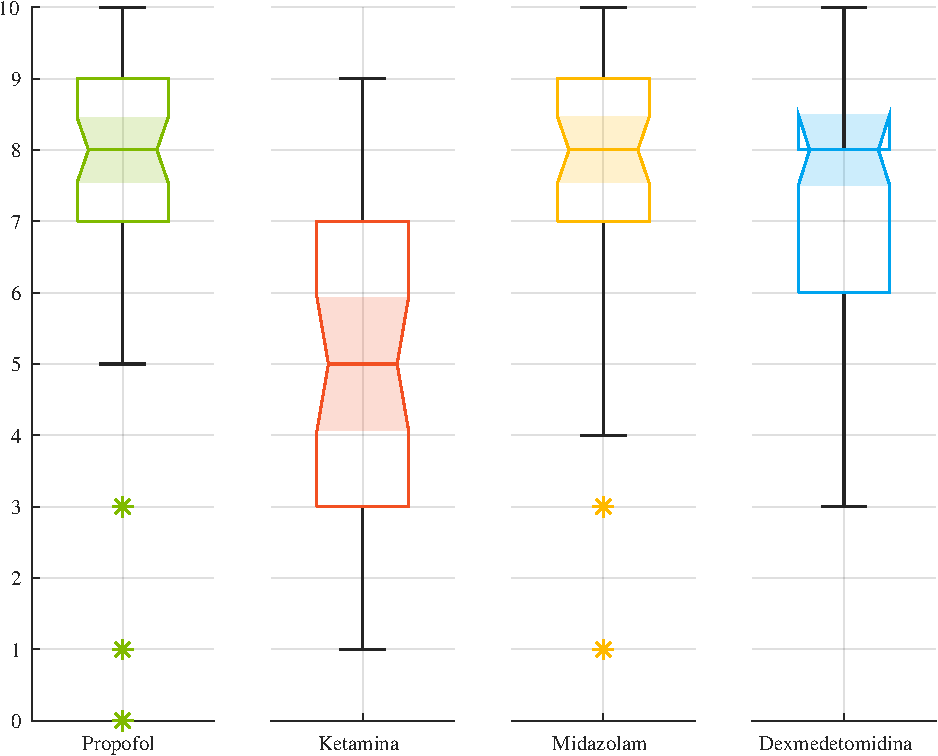
\includegraphics[width=0.8\textwidth]{Figure/qualita-colorful.pdf}
    \caption{Confronto del livello di soddisfazione percepito dagli infermieri (misurato in scala NRS) in relazione ai quattro agenti farmacologici testati in questo lavoro di tesi.}
    \label{fig:qualitascolorful}
\end{figure}

\begin{figure}[h]
    \centering
    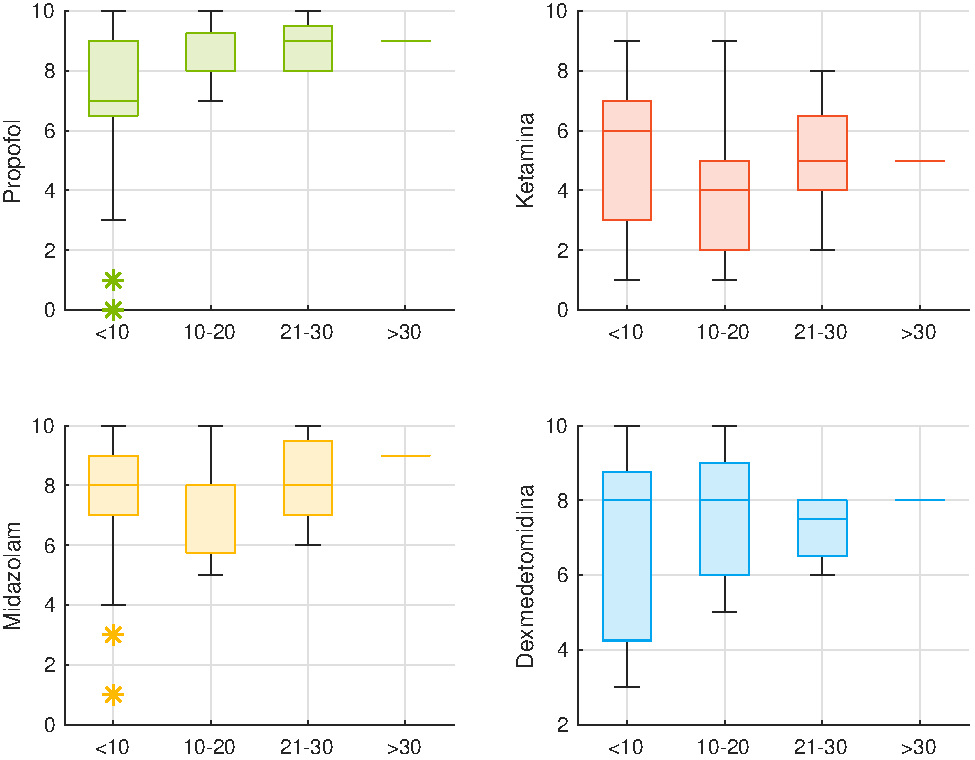
\includegraphics[width=1\textwidth]{Figure/qualita-stratificata.pdf}
    \caption{Livello di soddisfazione associato ai diversi agenti farmacologici (misurato secondo scala NRS) stratificato per il numero di sedazioni mensilmente assistite dagli intervistati.}
    \label{fig:qualitastratificata}
\end{figure}
\chapter{Discussione}

%\lipsum[1]
\chapter{Conclusioni}

%\lipsum[1]

\section*{Limiti}

%\lipsum[2]

%>APPENDICI
\begin{appendices}
\chapter{La sedazione procedurale}

La sedazione procedurale è una pratica sempre più diffusa ed utilizzata in una moltitudine di setting in tutto il mondo, anche da professionisti senza una formazione anestesiologica specifica. In ambito pediatrico, considerata l'importanza di offrire analgesia ed ansiolisi, tenendo conto anche delle tappe dello sviluppo psicofisico del bambino e al fine di prevenire la memoria di un vissuto negativo, viene quotidianamente eseguita per un vasto numero di procedure, sia in elezione che in urgenza. 

\section{Definizione}

La sedazione è uno stato di depressione della coscienza, con contestuale riduzione di vigilanza e consapevolezza, indotto dall'utilizzo di farmaci sedativi, ipnotici e dissociativi\footnote{I farmaci più comunemente utilizzati sono riportati nell'appendice B.} con o senza proprietà analgesiche. Questa condizione progredisce, senza una divisione arbitraria, lungo un \emph{continuum}: da un grado di sedazione minimo (o ansiolisi) ad un livello ben più profondo di anestesia generale, che richiede il supporto anestesiologico, attraversando le tappe della sedazione moderata e profonda \cite{Krauss2006}. \`E compito del sedatore conoscere le proprietà dei farmaci utilizzati e titolarli adeguatamente al fine di ottenere il livello di sedazione anticipatamente designato.  
\\Si definisce \emph{procedurale} quando viene attuata al di fuori del teatro operatorio per lo svolgimento di procedure diagnostiche e/o terapeutiche di breve durata, con il raggiungimento di un grado massimo di sedazione profonda e quindi con il mantenimento della funzionalità cardiorespiratoria e dei riflessi protettivi delle vie aeree, come la tosse e la deglutizione. 

Nonostante non esista un preciso confine tra un livello di sedazione ed il successivo, i principali stati di depressione della coscienza ottenibili possono essere descritti come segue~\cite{Statpearls, Berkenbosch2015}:

\begin{description}
\item[Analgesia] Trattamento del dolore senza alterazione intenzionale dello stato mentale.
\item[Sedazione minima] Anche detta ansiolisi; il paziente è sveglio e risponde normalmente allo stimolo verbale. Le funzioni cognitive e di coordinazione potrebbero essere minimamente alterate, mentre la funzionalità cardiorespiratoria non è influenzata.
\item[Sedazione moderata] Il paziente ha un livello di coscienza depresso ma risponde allo stimolo verbale, eventualmente accompagnato da una leggera sollecitazione tattile. Le vie aeree vengono mantenute pervie senza necessità di intervento e la funzionalità cardiorespiratoria è inalterata. 
\item[Sedazione profonda] Il paziente risulta difficilmente risvegliabile ma potrebbe rispondere a ripetuti stimoli verbali o dolorosi. Inoltre, potrebbe necessitare di supporto per mantenere le vie aeree pervie mentre la funzionalità cardiorespiratoria è solitamente inalterata. 
\item[Anestesia generale] Il paziente non è risvegliabile e necessita di supporto per mantenere le vie aeree pervie ed una ventilazione adeguata, infatti si accompagna solitamente a depressione respiratoria e cardiovascolare. 
\item[Sedazione dissociativa] La sedazione con ketamina rappresenta un'eccezione al continuum tra i diversi livelli di sedazione su cui si muovono gli altri agenti farmacologici. Infatti, i suoi effetti terapeutici sono correlati a specifici dosaggi, rappresentati nella tabella~\ref{tab:1}. Dal punto di vista sedativo, porta il paziente in uno stato catalettico, simile alla trance, in cui il paziente è insensibile agli eventi esterni e sperimenta profonda analgesia ed amnesia, tuttavia rimane sveglio e mantiene intatti la respirazione, i riflessi protettivi e la stabilità cardiopolmonare.

\end{description}

\section{Scopi}

I principali obiettivi per cui si effettuano le sedazioni procedurali sono \cite{Uptodatesed}: 

\begin{itemize}
    \item Garantire il benessere e l'incolumità del paziente durante tutte le fasi della procedura.
    \item Trattare l'ansia, indurre amnesia ed evitare un possibile trauma psicologico associato ad un'esperienza spiacevole e di difficile comprensione per il paziente pediatrico.
    \item Ridurre al minimo la percezione del dolore ed evitare un'eventuale risposta vagale alla procedura dolorosa.
    \item Limitare il movimento al fine di permettere una riuscita della procedura sicura ed efficace.

\end{itemize}

Questi scopi possono essere raggiunti al meglio utilizzando il farmaco al dosaggio più basso possibile che contestualmente consenta di ottenere l'effetto terapeutico desiderato \cite{Guidelines2019}.

\section{Formazione del sedatore}

Soprattutto in ambito pediatrico, per i motivi precedentemente esposti, c'è un ampia e crescente richiesta di figure qualificate, che possiedano le competenze adeguate a svolgere in sicurezza e con efficacia le sedazioni procedurali. Tale ruolo, storicamente di pertinenza dell'anestesista, viene sempre più praticato in tutto il mondo da una moltitudine di professionalità diverse. Da qui nasce l'esigenza di formare al meglio il personale incaricato dello svolgimento di tali sedazioni; nonostante non esistano ancora delle linee guida internazionalmente condivise sulle abilità di base che dovrebbe possedere un sedatore, ci sono due competenze chiave con cui tale professionista deve avere certamente destrezza: la gestione delle vie aeree e la rianimazione cardiopolmonare con supporto di defibrillatore. Parallelamente, un altro punto fondamentale che deve essere soddisfatto prima di procedere con la sedazione, riguarda la designazione di un team di emergenza, pronto ad intervenire in caso di complicanze che richiedano un livello di cure più avanzato.
\\Oltre a ciò ci sono alcune capacità e conoscenze che è importante facciano parte del bagaglio formativo del sedatore \cite{Simeupsedazione, Berkenbosch2015}: 
\begin{itemize}
    \item Deve essere in grado di individuare, durante la valutazione iniziale del paziente, gli elementi che possano indicare la necessità di supporto anestesiologico durante la procedura.
    \item Deve valutare il rischio di aspirazione del contenuto gastrico ed, in elezione, far rispettare un appropriato numero di ore di digiuno: minimo 2 ore per i liquidi chiari, 4 ore per il latte materno e 6 ore per il latte in formula o per pasti leggeri \cite{Guidelines2019}. 
    \item Deve conoscere l'anatomia respiratoria e i relativi volumi polmonari, che differiscono in base alle diverse età del bambino. 
    \item Deve avere familiarità con gli agenti sedativi ed analgesici più comunemente utilizzati, deve saperli titolare correttamente al fine di raggiungere il livello di profondità prefissato e saperne gestire gli eventuali effetti avversi. 
    \item Considerato il concetto di \emph{continuum} della sedazione, deve saper intervenire opportunamente se il livello di profondità ottenuto eccede quello desiderato e saper, quindi, gestire le conseguenti implicazioni respiratorie e cardiovascolari. 
    \item Deve saper leggere correttamente gli strumenti di monitoraggio, quali ad esempio pulsossimetria, capnografia ed elettrocardiografia, e saper interpretare i valori dei parametri vitali dei pazienti, sia in corso di procedura, sia in previsione della dimissione. 
    \item Deve saper intervenire prontamente in caso di perdita della pervietà delle vie aeree e della funzione ventilatoria. Pertanto è raccomandato che il sedatore abbia manualità con l'esecuzione della tecnica di intubazione endotracheale\footnote{\`E raccomandata l'attuazione di almeno 20 manovre di intubazione endotracheale in pazienti pediatrici, con supervisione di un anestesista, oltre ad almeno 30 sedazioni profonde altrettanto supervisionate \cite{Simeupsedazione}.}.
\end{itemize}

\section{Valutazione preprocedurale}

Nella fase di pianificazione della sedazione risulta fondamentale instaurare una relazione di fiducia con i genitori del bambino e discutere insieme dei rischi, dei benefici, degli effetti attesi e di eventuali reazioni avverse rispetto alla procedura ed alla sedazione, al fine di ottenere un appropriato consenso informato. Oltre a ciò è necessario raccogliere un'approfondita anamnesi familiare, patologica prossima e remota, con l'obiettivo di individuare i pazienti nei quali è necessario procedere con il supporto anestesiologico. In questa fase andranno indagate eventuali allergie a farmaci e alimenti, precedenti reazioni avverse in corso di anestesia o sedazione, la presenza di rilevanti patologie pregresse o croniche e i farmaci assunti quotidianamente, con particolare attenzione a patologie della sfera polmonare, quali asma o bronchiti asmatiformi; infine una possibile storia di russamento o apnee notturne e/o una condizione di obesità possono correlare con un maggior rischio di ostruzione delle vie aeree \cite{Simeupsedazione, Guidelines2019}.
Convenzionalmente, per determinare il rischio anestesiologico si utilizza la classificazione della \emph {American Society of Anesthesiologists} (ASA), riportata nella tabella \ref{tab:ASA}: possono essere sedati in sicurezza i bambini con i profili ASA I e II, anche ASA III, quando si tratta di soggetti con particolari patologie (ad esempio leucemia) in condizioni cliniche stabili e in assenza di ulteriori fattori di rischio. 

\bigskip

\bgroup
\def\arraystretch{1.5}
\begin{table}[!ht]
    \centering
    \begin{tabular}{p{0.08\textwidth}|p{0.3\textwidth}|p{0.25\textwidth}|p{0.25\textwidth}}
    
       \textit{\footnotesize Classe}     &  \textit{\footnotesize Condizioni cliniche} & \textit{\footnotesize Esempi di patologie} & \textit{\footnotesize Idoneità alla sedazione}\\ \hline\hline
       {\footnotesize ASA I} & {\footnotesize Paziente sano} & {\footnotesize Nessuna} & {\footnotesize Eccellente} \\ \hline
       {\footnotesize ASA II} & {\footnotesize Paziente con patologia sistemica lieve --- senza limitazioni funzionali significative} & {\footnotesize asma lieve, epilessia in trattamento, anemia, diabete controllato} & {\footnotesize Generalmente buona}\\ \hline
       {\footnotesize ASA III} & {\footnotesize Paziente con patologia sistemica severa --- con relative limitazioni funzionali} & {\footnotesize Asma moderata-severa, epilessia farmacoresistente, polmonite, diabete incontrollato, obesità moderata, prematurità} & {\footnotesize Da media a scarsa: considerare i rischi in relazione ai benefici}\\ \hline
       {\footnotesize ASA IV} & {\footnotesize Paziente con patologia sistemica severa, che rappresenta una costante minaccia per la vita} & {\footnotesize Severa displasia broncopolmonare, sepsi, avanzata insufficienza polmonare, cardiaca, epatica, renale o endocrina} & {\footnotesize Scarsa: i benefici raramente superano i rischi} \\ \hline
       {\footnotesize ASA V} & {\footnotesize Paziente moribondo con ridotte possibilità di sopravvivenza senza intervento chirurgico} & {\footnotesize Trauma severo, shock settico, MODS\tablefootnote{\emph{Multiple Organ Dysfunction Syndrome}}, aneurisma aortico, ischemia intestinale} & {\footnotesize Estremamente scarsa}\\ \hline
       {\footnotesize ASA VI} & {\footnotesize Paziente con morte cerebrale dichiarata destinato alla donazione di organi} & & \\ 
       
    \end{tabular}
    \caption{Classificazione della \emph{American Society of Anesthesiologists}, adattata da \cite{Krauss2006, Simeupsedazione, Daud2014}.}
    \label{tab:ASA}
\end{table}
\egroup



Successivamente si valutano l'età ed il peso del bambino, elementi fondamentali per la scelta farmacologica, i parametri vitali e si esegue un'esame obiettivo accurato, prestando particolare attenzione all'ispezione del cavo orale, con lo scopo di individuare un'eventuale presenza di ipertrofia tonsillare o di anomalie anatomiche e di predire la difficoltà di posizionamento del tubo endotracheale, manovra che può rendersi necessaria e salvifica in caso di complicanze in corso di procedura \cite{Guidelines2019}. Per tale scopo viene utilizzata la scala di Mallampati che definisce, in base all'anatomia del cavo orale, quattro stadi in ordine crescente di complessità di manovra, descritti in seguito e mostrati nella figura \ref{fig:mallampati}:

\begin{itemize}
    \item Classe I: piena visibilità dei pilastri tonsillari, dell'ugola e del palato molle, è associata ad una difficoltà di intubazione bassa.
    \item Classe II: visibilità del palato duro, del palato molle e della porzione superiore di tonsille ed ugola.
    \item Classe III: visibilità di palato molle e palato duro.
    \item Classe IV: visibilità esclusiva del palato duro a causa della frapposizione della lingua, è associata ad un'elevata difficoltà di intubazione, che può richiedere la presenza di una mano esperta. 
\end{itemize}

\bigskip

\begin{figure}[h]
    \centering
    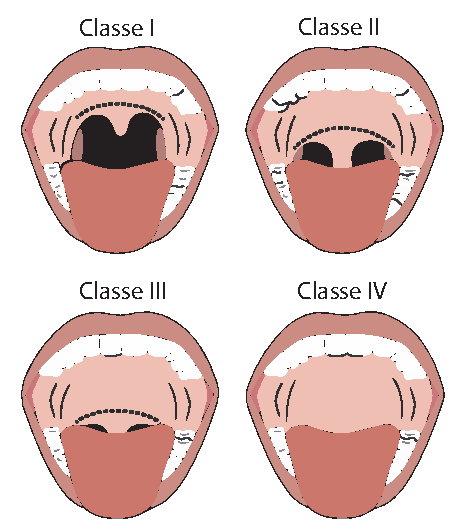
\includegraphics[width=0.6\textwidth]{Figure/mallampatpdf.pdf}
    \caption{Classificazione di Mallampati, adattata da \cite{Vargo2012}.}
    \label{fig:mallampati}
\end{figure}

\newpage

\section{Ambiente ed equipaggiamento}

Prima di procedere con la sedazione è indispensabile valutare l'idoneità dell'ambiente e del materiale, necessario per il monitoraggio del paziente o in caso di complicanze. \`E, quindi, importante assicurarsi sia che ci sia spazio a sufficienza attorno al paziente, in modo tale da poter intervenire agilmente con eventuali manovre rianimatorie o garantendo un'adeguata ventilazione in caso ad esempio di apnea o laringospasmo, sia che la strumentazione per il monitoraggio e la gestione delle vie aeree e del circolo sia presente e funzionante e i farmaci d'emergenza prontamente reperibili. 

L'equipaggiamento da avere sempre a disposizione e da esaminare in termini di quantità e qualità prima di ogni sedazione può essere raggruppato in sei categorie, facilmente memorizzabili grazie all'acronimo inglese \texttt{SOAPME}, descritto nella tabella \ref{tab:soapme}.

\bgroup
\def\arraystretch{1.5}
\begin{table}[!h]
    \centering
    \begin{tabular}{p{0.05\textwidth} p{0.3\textwidth} p{0.6\textwidth}}
       
       \texttt{S} & Aspirazione (\emph{Suction}) & Sondini da aspirazione di dimensione adeguata ed un aspiratore funzionante \\ \hline
      \texttt{O} & Ossigeno & Erogatore di ossigeno a muro collegato ad un pallone va e vieni con una maschera della misura del paziente. Inoltre, è raccomandata la disponibilità di una bombola con ossigeno sufficiente a garantire, in caso di complicanze, il trasporto del paziente verso la struttura di emergenza e rianimazione di riferimento o in alternativa un pallone ambu\\ \hline
       \texttt{A} & Vie aeree (\emph{Airway}) & Equipaggiamento per la gestione delle vie aeree: cannule oro o nasofaringee, maschere laringee, set di intubazione. Tutto il materiale deve essere di dimensioni appropriate all'anatomia del paziente\\ \hline
       \texttt{P} & Farmaci (\emph{Pharmacy)} & Tutti i farmaci fondamentali al supporto vitale del paziente in situazioni di emergenza, quali ad esempio adrenalina, amiodarone, atropina, beclometasone, salbutamolo e flumazenil (antagonista del recettore GABA\ped{A})\\ \hline
       \texttt{M} & Monitoraggio & Strumenti indispensabili al monitoraggio del paziente, quali saturimetro (con segnale acustico), capnografo, stetofonendoscopio e sfigmomanometro, monitor ECG\tablefootnote{Il monitoraggio elettrocardiografico non è richiesto in assenza di patologie cardiovascolari poiché non modifica il decorso e gli esiti della sedazione e/o dell'analgesia \cite{Krauss2006}.}\\ \hline
       \texttt{E} & Equipaggiamento & Disponibilità di un carrello o zaino di emergenza e di un defibrillatore\\
    \end{tabular}
    \caption{\texttt{SOAPME}: check list del materiale, adattata da \cite{Daud2014, Guidelines2019}.}
    \label{tab:soapme}
\end{table}
\egroup

Oltre a ciò, è imprescindibile la presenza di almeno due professionisti sanitari durante la procedura, solitamente un medico ed un infermiere. Mentre il primo sceglie i sedativi da utilizzare ed esegue la procedura, il secondo ha il compito di controllare i parametri vitali ed i segni clinici del paziente, oltre a somministrare i farmaci \cite{Krauss2006, Simeupsedazione}. 

\section{Monitoraggio del paziente}

Il monitoraggio del paziente è fondamentale ai fini dello svolgimento di una sedazione procedurale in totale sicurezza: permette infatti di riconoscere tempestivamente eventuali complicanze, tra le più rilevanti le alterazioni cardiorespiratorie. 
Per quanto riguarda la sedazione da moderata a profonda, il monitoraggio del paziente include \cite{Krauss2006, Simeupsedazione}: 

\begin{itemize}
    \item L'osservazione continua del volto, della bocca e dei movimenti del torace del paziente, con l'obiettivo di individuare precocemente eventuali alterazioni nella dinamica respiratoria, possibili apnee o la comparsa di laringospasmo o di secrezioni.
    \item Misurazione continua e registrazione in vari tempi dei parametri vitali del paziente: la frequenza cardiaca e respiratoria, la saturazione e la pressione arteriosa vanno rilevate prima di cominciare la procedura, ad intervalli regolari durante la stessa e fino a completo risveglio. 
    \item Rilevazione dell'\emph{end tidal CO\ped{2}} o anidride carbonica di fine espirio tramite capnografia.
    \item Continua valutazione del grado di profondità della sedazione tramite l'utilizzo di scale appositamente designate, quali ad esempio l'\emph{Aldrete score} o la \emph{Pediatric Sedation State Scale}.
\end{itemize} 

I punti critici della sedazione, in cui andrebbe posta particolare attenzione, sono rappresentati dai momenti successivi alla somministrazione dei farmaci e dalle fasi immediatamente seguenti il termine della procedura poiché, una volta rimossi gli stimoli dolorosi e tattili, si potrebbe verificare un incremento del livello di profondità con possibili e temibili complicanze, quali la depressione respiratoria \cite{Daud2014}. 
\\Inoltre, tutti i parametri rilevati e il livello di sedazione raggiunto vanno poi opportunamente registrati in una scheda di sedazione dove vengono riportati insieme ai dati anagrafici, ai dosaggi dei farmaci somministrati compresi di ora e di via di somministrazione, l'ossigeno supplementare erogato, l'ora di inizio e fine della procedura e le eventuali reazioni avverse \cite{Guidelines2019, Simeupsedazione}. 


\subsection*{Capnografia}
Soprattutto in corso di sedazione profonda, risulta indispensabile l'utilizzo del capnografo, uno strumento in grado di dare informazioni in tempo reale sullo stato ventilatorio del paziente. L'uso del solo pulsossimetro sarebbe infatti inappropriato, in quanto si tratta di un dispositivo che misura la saturazione di ossigeno nel sangue ma non dà indicazioni sui livelli di anidride carbonica e presenta un tempo di latenza variabile (dipendente dall'età, dalle condizioni cliniche del paziente e dalla somministrazione di ossigeno) tra l'inizio di un'eventuale apnea o ipoventilazione e la rilevazione della conseguente desaturazione \cite{Long2017}. Il capnografo, invece, permette di misurare in modo non invasivo la pressione parziale della CO\ped{2} nell'aria espirata e di fornire una rappresentazione grafica dell'andamento ondulatorio della concentrazione della CO\ped{2} in relazione al tempo \cite{Baruch2005}. Analizzando la curva capnografica e il valore dell'\emph{end tidal CO\ped{2}} misurato dallo strumento, ovvero la concentrazione della CO\ped{2} di fine espirio, è possibile individuare repentinamente e con anticipo rispetto al pulsossimetro eventuali alterazioni ventilatorie, quali depressione respiratoria o apnea ma anche ostruzione delle vie aeree superiori, laringospasmo e broncospasmo \cite{Long2017}. I tracciati caratteristici di queste condizioni sono schematicamente rappresentati nelle figure \ref{fig:apnea}, \ref{fig:laringo}, \ref{fig:bronco}.
Nei soggetti sani, invece, la curva capnografica ha una forma rettangolare e consiste in quattro fasi, rappresentate nella figura \ref{fig:curvacapno} e descritte in seguito \cite{Uptodatecapno}: 

\begin{figure}[t]
    \centering
    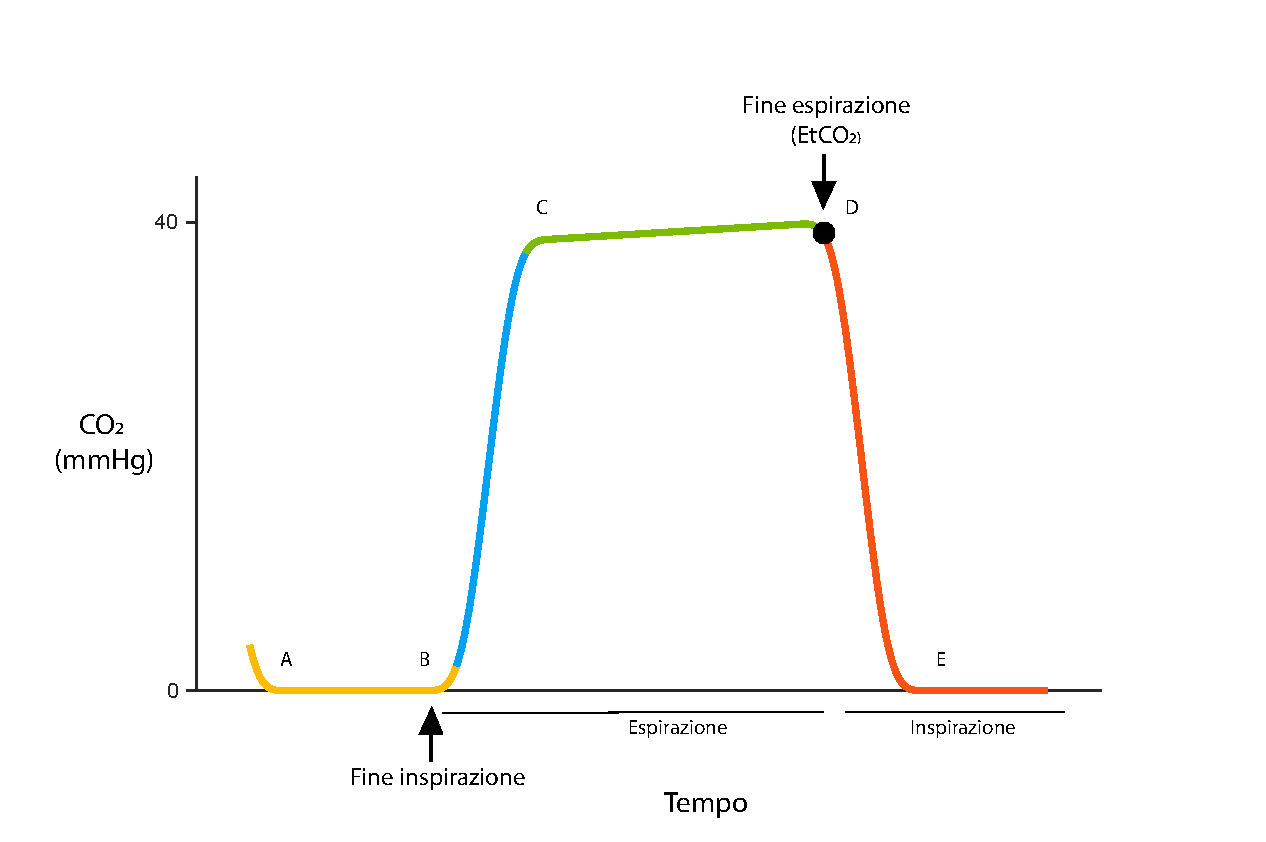
\includegraphics[width=1\textwidth]{Figure/capnopdf1.pdf}
    \caption{Il normale aspetto della curva capnografica.}
    \label{fig:curvacapno}
\end{figure}

\begin{fancybox}{giallomicrosoft}
    \textsc{Fase 1} \small{(da A a B)}: è rappresentata da una linea isoelettrica, identifica il tempo intercorso tra la fine dell’inspirio e l’inizio dell’espirazione: in questo periodo fuoriesce l'aria dallo spazio morto fisiologico, che non partecipando agli scambi alveolari non contiene CO\ped{2}.
\end{fancybox}

\begin{fancybox}{blumicrosoft}
\textsc{Fase 2} \small{(da B a C)}: è identificata da una linea ascendente che ritrae il passaggio della CO\ped{2} dagli alveoli alle vie aeree superiori e quindi l'espirazione di gas alveolari misti a quelli dello spazio morto, consegue un rapido incremento della concentrazione di CO\ped{2} espirata.
    
\end{fancybox}

\begin{fancybox}{verdemicrosoft}
\textsc{Fase 3} \small{(da C a D)}: anche chiamata \emph{plateau alveolare}, si tratta dell'arco di tempo in cui la concentrazione di CO\ped{2} raggiunge un livello uniforme durante l'intero flusso espiratorio dagli alveoli al naso. Il punto D delinea la fine dell'espirazione e il momento di massima concentrazione di CO\ped{2}, definito \emph{end tidal CO\ped{2}} (EtCO\ped{2}) e visualizzabile numericamente sullo schermo del capnografo (valori normali sono compresi tra 35 e 45 mmHg).

\end{fancybox}

\begin{fancybox}{rossomicrosoft}
\textsc{Fase 4} \small{(da D ad E)}: a questo punto comincia il ciclo inspiratorio e la CO\ped{2} torna sulla linea dello zero. 

\end{fancybox}

\begin{comment}
\begin{itemize}
    \item {\fcolorbox{black}{giallomicrosoft}{\texttt{Fase 1}}} \small{(da A a B)}: è rappresentata da una linea isoelettrica, identifica il tempo intercorso tra la fine dell’inspirio e l’inizio dell’espirazione: in questo periodo fuoriesce l'aria dallo spazio morto fisiologico\footnote{Lo spazio morto fisiologico è la frazione d'aria del volume corrente intrappolata nelle vie aeree di conduzione, che non partecipa agli scambi gassosi.}, che non partecipando agli scambi alveolari non contiene CO\ped{2}.
    \item {\fcolorbox{black}{blumicrosoft}{\texttt{Fase 2}}} \small{(da B a C)}: è identificata da una linea ascendente che ritrae il passaggio della CO\ped{2} dagli alveoli alle vie aeree superiori e quindi l'espirazione di gas alveolari misti a quelli dello spazio morto, consegue un rapido incremento della concentrazione di CO\ped{2} espirata.
    \item {\fcolorbox{black}{verdemicrosoft}{\texttt{Fase 3}}} \small{(da C a D)}: anche chiamata \emph{plateau alveolare}, si tratta dell'arco di tempo in cui la concentrazione di CO\ped{2} raggiunge un livello uniforme durante l'intero flusso espiratorio dagli alveoli al naso. Il punto D delinea la fine dell'espirazione e il momento di massima concentrazione di CO\ped{2}, definito \emph{end tidal CO\ped{2}} (EtCO\ped{2}) e visualizzabile numericamente sullo schermo del capnografo (valori normali sono compresi tra 35 e 45 mmHg).
    \item {\fcolorbox{black}{rossomicrosoft}{\texttt{Fase 4}}} \small{(da D ad E)}: a questo punto comincia il ciclo inspiratorio e la CO\ped{2} torna sulla linea dello zero. 
    
\end{itemize}
\end{comment}



\section{Preossigenazione}

Una pratica raccomandata in caso di sedazioni da moderate a profonde consiste nella preossigenazione del paziente, ovvero la somministrazione, prima dell'induzione farmacologica, di un'elevata frazione inspiratoria di ossigeno (FiO\ped{2}). In questo modo è possibile ritardare da 2 a 4 minuti gli effetti di un'eventuale ipopnea od apnea sulla saturazione dell'emoglobina: la preossigenazione consente infatti di aumentare le riserve di ossigeno del nostro organismo e di favorire il washout dell'azoto alveolare (N\ped{2}). Questi risultati si riflettono in termini di aumento della frazione alveolare dell'ossigeno (FaO\ped{2}), della pressione parziale dell'ossigeno nel sangue (PaO\ped{2}) e della contestuale riduzione della frazione alveolare dell'azoto (FaN\ped{2}) \cite{Nimmagadda2017}.
I limiti di questa manovra, invece, risiedono nell'aumento dell'ansia preprocedurale, soprattutto nei bambini più piccoli, e nel possibile ritardo del riconoscimento delle alterazioni ventilatorie; per tale motivo è consigliato il contemporaneo utilizzo del capnografo e/o la stretta e continua osservazione diretta dei movimenti toracici del paziente \cite{Fu2004}. 
\\Oltre alla preossigenazione, anche durante la procedura è fortemente consigliato l'utilizzo di ossigeno supplementare, erogato attraverso il sistema di pallone va e vieni (anche detto \emph{da anestesia}), in modo tale da poter sia modulare la pressione di ventilazione in base alle necessità ed all'elasticità del torace del paziente, sia garantire un supporto ventilatorio adeguato in caso di arresto respiratorio, chiudendo la valvola e fornendo pressione positiva \cite{Simeupsedazione}.

\section{Eventi avversi}

Le complicanze associate alla sedazione procedurale possono essere suddivise in eventi maggiori, quali la morte, i danni neurologici e l'arresto cardiopolmonare e in eventi minori, sia di natura respiratoria quali l'ipossia, l'apnea, il laringospasmo, il broncospasmo e la rigidità toracica; sia di natura cardiovascolare, ad esempio ipo- o ipertensione e bradicardia. Gli effetti avversi maggiori sono estremamente rari e spesso associati ad un monitoraggio clinico inadeguato ed incostante, una valutazione preprocedurale poco attenta, un setting non appropriato e l'assenza di un sistema di emergenza pronto ad intervenire in caso di necessità \cite{Uptodatesed}.
Riporto sotto il dettaglio di alcune delle complicanze più frequenti.

\newpage

\begin{description}
\item[Ipossia] Si tratta di una riduzione del livello di ossigenazione del sangue, che può essere convenzionalmente definita con valori di saturazione dell'emoglobina inferiori al 94$\%$ in aria ambiente o con una pressione parziale dell'ossigeno (PaO\ped{2}) inferiore a 60 mmHg. I meccanismi che portano all'ipossia in corso di sedazione procedurale sono principalmente due: l'instaurarsi di un'ipoventilazione centrale dovuta alla depressione respiratoria causata dall'azione farmacologica e l'ostruzione delle vie aeree superiori dovuta o a perdita di tono della muscolatura faringea con conseguente caduta posteriore della lingua o alla presenza di secrezioni abbondanti. Il monitoraggio capnografico e l'osservazione attiva del torace del paziente permette di riconoscere prontamente e distinguere queste situazioni. In caso di mancata risoluzione spontanea, se la causa è l'ipossia centrale si potrà solo ossigenare e ventilare adeguatamente il paziente in attesa del ripristino della normale autonomia respiratoria, se si tratta invece di ipossia secondaria ad ostruzione si potrà intervenire aspirando le vie aeree, posizionando correttamente il capo: in iperestensione nei bambini sopra l'anno e in posizione neutra nei lattanti. A discrezione, si può procedere posizionando una cannula orofaringea o somministrando atropina in caso di eccessive secrezioni o bradicardia riflessa conseguente all'aspirazione \cite{Simeupsedazione}. 

\item[Apnea] \`E definita come assenza di ventilazione per almeno 20 secondi ed è rappresentata da una linea piatta sul monitor capnografico. Poiché rappresenta l'evoluzione finale degli stessi meccanismi che portano all'ipossia, si può suddividere anch'essa in primaria e secondaria. Un'attenta osservazione clinica del paziente permette di distinguere facilmente le due forme: nel primo caso i movimenti toracici risulteranno ridotti o assenti, mentre nel secondo caso appariranno accentuati al fine di vincere l'ostacolo. Se si verifica tale complicanza è necessario intervenire stimolando il paziente con sollecitazioni dolorose, riposizionando il capo, aspirando, ossigenando e ventilando come descritto sopra per l'ipossia \cite{Simeupsedazione}. 

\begin{figure}[h]
    \centering
    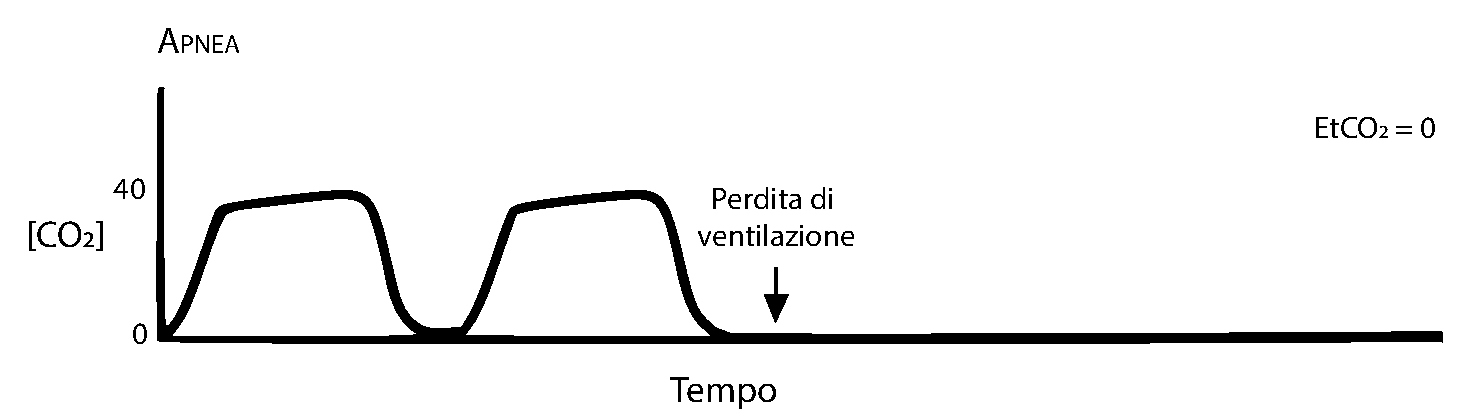
\includegraphics[width=0.8\textwidth]{Figure/apnea.png}
    \caption{Tracciato capnografico tipico di un'apnea, adattato da \cite{Baruch2005}.}
    \label{fig:apnea}
\end{figure}


\item[Laringospasmo] \`E un fenomeno piuttosto raro, con un'incidenza attorno all'1$\%$, dovuto ad una completa adduzione delle corde vocali tale da rendere impossibile il passaggio dell'aria. \`E più spesso associato alla somministrazione di ketamina o all'esecuzione di procedure che stimolino le vie aeree superiori, quale la gastroscopia. Per tentare di superare l'ostruzione è possibile riposizionare il capo, somministrare ossigeno ad alti flussi e ventilare il paziente con pallone ambu o va e vieni a valvola chiusa. Qualora non sia sufficiente si può considerare di sublussare la mandibola per migliorare la pervietà delle vie aeree, approfondire il livello di sedazione e frattanto chiamare l'anestesista \cite{Simeupsedazione}. 

\begin{figure}[h]
    \centering
    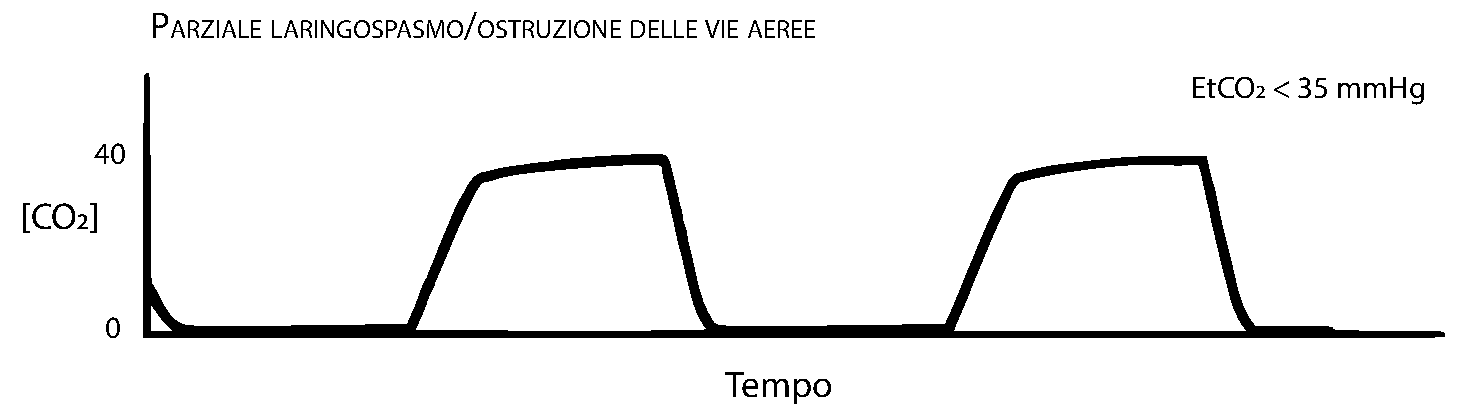
\includegraphics[width=0.8\textwidth]{Figure/laringospasmo.png}
    \caption{Tracciato capnografico tipico di un parziale laringospasmo, adattato da \cite{Baruch2005}.}
    \label{fig:laringo}
\end{figure}

\item[Broncospasmo] \`E caratterizzato dalla contrazione della muscolatura liscia dei bronchi e bronchioli, con conseguente riduzione del calibro bronchiale e dell'afflusso di aria agli alveoli. Si verifica più frequentemente nei pazienti asmatici noti o nei bambini che hanno avuto recentemente un'infezione delle vie aeree. In questi casi è possibile prevenirlo mediante l'utilizzo di salbutamolo per via inalatoria o, qualora possibile, scegliendo come sedativo la ketamina, che possiede parziale azione broncodilatante, o altre molecole che non interferiscano con il sistema respiratorio \cite{Simeupsedazione}.

\begin{figure}[h]
    \centering
    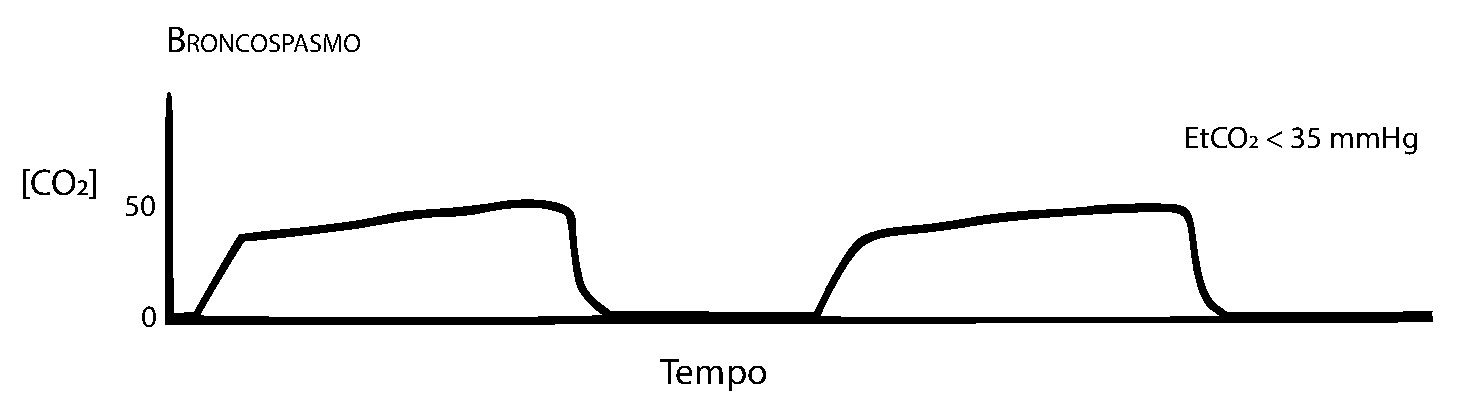
\includegraphics[width=0.8\textwidth]{Figure/broncospasmo.png}
    \caption{Tracciato capnografico tipico di un broncospasmo, adattato da \cite{Baruch2005}.}
    \label{fig:bronco}
\end{figure}

\end{description}

\section{Risveglio e dimissione}

Al termine della procedura il paziente va collocato in un ambiente protetto e i suoi parametri vitali vanno monitorati fino al completo risveglio, ovvero fino a quando non ha ripreso un livello di consapevolezza appropriato per l'età e quindi non è più a rischio di depressione cardiorespiratoria \cite{Krauss2006}. Circa 30 minuti dopo che il paziente ha ricominciato le sue normali attività, parla e rimane seduto senza aiuto, è possibile somministrargli un po' di acqua e successivamente anche piccole quantità di cibo. Il bambino può essere dimesso in sicurezza quando sono soddisfatti i seguenti criteri \cite{Uptodatesed, Simeupsedazione}: 
\begin{itemize}
    \item Le vie aeree sono pervie e la funzione cardiovascolare stabile
    \item Il paziente è vigile e i riflessi protettivi delle vie aeree intatti (vomito, tosse, deglutizione)
    \item Il bambino ha ricominciato a muoversi in maniera appropriata alla sua età e al suo stato di sviluppo psicofisico, inoltre riesce a mantenere lo stato di veglia senza difficoltà
    \item \`E adeguatamente idratato e la nausea e il vomito sono assenti o controllati dalla terapia
    \item Non ha cefalea o segni neurologici
    \item Non ha dolore oppure esso viene trattato in maniera appropriata ed efficace
\end{itemize}
\chapter{I farmaci}

Al fine di garantire un'ottima riuscita della procedura ed evitare nel bambino il ricordo di un'esperienza spiacevole e talora traumatica, ad oggi si può ricorrere sia ad interventi farmacologici di analgosedazione che ad interventi non farmacologici. Quest'ultimi possono essere utilizzati come metodo complementare o esclusivo, con innumerevoli benefici: dal ridurre l'agitazione preprocedurale e permettere una miglior transizione alla fase di sedazione, al contenere le dosi di farmaco utilizzate nel corso della procedura finanche, in alcuni casi, al prevenire del tutto il ricorso alla sedazione \cite{Uptodate}. Si tratta di approcci cognitivi e comportamentali che racchiudono tecniche di distrazione, rilassamento, desensibilizzazione e rinforzo positivo; risulta inoltre fondamentale, al fine di abbassare i livelli di ansia, instaurare una relazione di fiducia con i genitori e il bambino e definire un'adeguata strategia comunicativa, che adotti un linguaggio adeguato all'età o eventualmente introduca il gioco come strumento per prendere confidenza con le attrezzature mediche e le varie fasi della procedura. Tuttavia la sedazione farmacologica rimane la principale risorsa per agevolare le procedure più invasive. 

La scelta dell'agente farmacologico incide fortemente sulla qualità del risveglio post procedurale e va basata su diversi fattori. Premesso che il farmaco o la combinazione di farmaci selezionati deve indurre sedazione e analgesia adeguate a consentire il completamento della procedura con successo, mantenendo i riflessi protettivi delle vie aeree e l'autonomia cardiorespiratoria \cite{Krauss2006}, nel processo di decisione è importante valutare anche il livello di profondità della sedazione desiderato, conseguenza a sua volta del grado di analgesia richiesto dalla procedura. Infatti, talvolta è sufficiente solamente l'ansiolisi, altre volte è necessaria una più estesa analgesia, in altre occasioni invece lo scopo è quello di mantenere il paziente immobile, senza quindi bisogno di trattare il dolore. Altri elementi che guidano nella scelta del farmaco sono la familiarità nell'utilizzo da parte del sedatore e le caratteristiche individuali del paziente (età, comorbidità, allergie, grado di collaborazione, {\color{orange} ore di digiuno (?)}), che possono controindicare alcuni agenti farmacologici \cite{Uptodate}.
Infine, sono rilevanti alcune caratteristiche farmacocinetiche: sono infatti preferenziali farmaci con molteplici vie di somministrazione, induzione rapida e breve emivita, tale da concedere un celere recupero con assenti o minimi effetti collaterali.

Di seguito verranno dunque analizzate e confrontate le proprietà, i dosaggi, le indicazioni e gli effetti collaterali dei farmaci più comunemente utilizzati al di fuori della sala operatoria. 

\section{Propofol}

Il propofol è un sedativo ipnotico, non analgesico, il cui meccanismo d'azione a livello del sistema nervoso centrale non è del tutto noto, anche se ne è stata studiata l'interazione con il recettore A dell'acido $\gamma$-amminobutirrico (GABA) \cite{Propofol2015}.

\subsection*{Farmacodinamica}

Il legame tra le molecole di propofol e il recettore ionotropico GABA-A è responsabile degli effetti centrali del farmaco. Questo recettore è costituito da un complesso proteico associato ad un canale per il cloro ed è presente a livello postsinaptico di molti neuroni. Una volta riconosciuto il ligando, si verifica un aumento del flusso degli ioni cloro attraverso la membrana, determinando iperpolarizzazione del neurone ed un conseguente effetto inibitorio, con minor eccitabilità e risposta agli stimoli esterni \cite{Propofol2015}.

\subsection*{Farmacocinetica}

Uno dei motivi per cui il propofol è ampiamente utilizzato riguarda proprio le sue vantaggiose caratteristiche farmacocinetiche: ha infatti un esordio d'azione estremamente rapido (30-45 secondi) ed un altrettanto rapido risveglio (5-15 minuti dopo singolo bolo, più lento in caso di infusione continua o boli multipli) \cite{Simeupsedazione, Uptodatepharmacology}. Si tratta di una molecola liposolubile, che supera la barriera ematoencefalica, macroscopicamente il propofol assume un aspetto lattescente e può essere somministrato solo per via endovenosa. Nel momento dell'iniezione può causare bruciore locale, che può essere prevenuto utilizzando una vena di calibro maggiore o diluendo a metà il propofol con soluzione fisiologica (5 mg/mL) \cite{Simeupsedazione}. 

\subsection*{Posologia}

Viene somministrato con un dosaggio di 1-2 mg/kg come bolo iniziale d'induzione, seguito da successivi boli multipli da 0.5 a 1 mg/kg ogni 2-3 minuti. Per le procedure più lunghe può anche essere utilizzato in infusione continua.
La dose massima è di 10 mg/kg totali per procedura \cite{Simeupsedazione}.

\subsection*{L'associazione con la ketamina}

Se la procedura è dolorosa il propofol può essere dato in combinazione con la ketamina, che oltre ad avere un'importante azione analgesica controbilancia gli effetti ipotensivo e bradicardizzante del propofol. Esistono in commercio delle formulazioni chiamate \emph{ketofol} con diversi rapporti di ketamina e propofol, tra i vantaggi risalta anche una minor incidenza di vomito e agitazione al risveglio, poiché l'effetto combinato permette di risparmiare ketamina \cite{Simeupsedazione}.

\subsection*{Effetti collaterali}

I principali effetti collaterali del propofol sono rappresentati dalla depressione respiratoria e dalla conseguente apnea, che dipendono dal dosaggio, dalla velocità di somministrazione e dalla risposta soggettiva del paziente. Inoltre, il propofol può determinare ipotensione e più raramente bradicardia \cite{propofolsafety2010}.
Un altro temibile quanto raro effetto avverso è costituito dalla \emph{sindrome da infusione di propofol}, potenzialmente fatale e descritta sia negli adulti che nei bambini \cite{Propofolinfusionsyndrome2019}. Si tratta di un insieme di segni e sintomi che si verifica in pazienti critici, che ricevono propofol in infusione a dosaggi elevati (>5 mg/kg/h) o per un periodo prolungato (>48h) ed è caratterizzata dalla presenza di una o più delle seguenti alterazioni, non spiegabili altrimenti: acidosi metabolica, rabdomiolisi, variazioni elettrocardiografiche associate o meno ad AKI, iperkaliemia, dislipidemia, scompenso cardiaco, febbre, elevazione degli enzimi epatici o del lattato. 

\section{Ketamina}

La ketamina è un farmaco anestetico dissociativo derivato dalla fenilciclidina con potenti proprietà sedative, analgesiche ed amnesiche. E' stato introdotto in commercio per la prima volta nel 1970 e da allora viene largamente utilizzato per lo più in ambito anestesiologico ma possiede un'ampia gamma di possibili applicazioni cliniche \cite{Ketamineapplication2019}: dal trattamento del dolore cronico, anche in pazienti oncologici, al trattamento del disturbo depressivo maggiore, grazie ai suoi effetti antidepressivo ed antisuicidario. Inoltre, mentre rimane controverso il suo ruolo nel trattamento dell'asma, sono riconosciute le sue azioni antinfiammatoria ed immunomodulatrice, a cui si aggiungono quella antiproliferativa ed apoptotica, che vengono studiate con interesse per la ricerca sulla soppressione tumorale.

\subsection*{Farmacodinamica}

La ketamina è un farmaco che porta il paziente in uno stato dissociativo, simile alla trance, in cui l'individuo rimane parzialmente vigile ma con una depressione della consapevolezza: mantiene infatti gli occhi aperti ma non interagisce con l'ambiente circostante e non percepisce dolore. A differenza di altri farmaci non presenta un \emph{continuum della sedazione}, piuttosto l'effetto è presente o assente a seconda del dosaggio. Viene scelta per la sua ottima capacità analgesica e l'alto profilo di sicurezza, in quanto permette il mantenimento dei riflessi protettivi delle vie aeree e non deprime il centro del respiro; inoltre dal punto di vista cardiovascolare aumenta la frequenza cardiaca e la pressione arteriosa \cite{Krauss2006}. 
\\La ketamina esercita le sue proprietà attraverso l'interazione con diversi recettori. Tuttavia, la maggior parte degli effetti sono dovuti al blocco dei recettori NMDA (\emph{N-Metil-D-Aspartato}, ai quali il farmaco si lega come antagonista non competitivo. Si tratta di canali ionici glutammatergici permeabili agli ioni calcio, i quali normalmente sono implicati nell'attivazione di diversi pathway intracellulari \cite{Zanos2018}.
\\La ketamina esiste sotto forma di due enantiomeri \footnote{Sono isomeri ottici, ovvero entità molecolari speculari e non sovrapponibili.} :levogiro (S) e destrogiro (R). La forma levogira ha un maggior attività anestetica ed analgesica, favorisce una miglior immobilità del paziente e un recupero più rapido, mentre la forma destrogira è più efficace per l'uso antidepressivo \cite{Simeupsedazione}.

\subsection*{Farmacocinetica}

La ketamina è altamente liposolubile, si distribuisce ai tessuti periferici e supera rapidamente la barriera ematoencefalica. Viene preferenzialmente somministrata per via endovenosa o intramuscolare ma, seppur con una biodisponibilità inferiore, può essere utilizzata anche attraverso altre vie: intranasale, rettale ed orale. \cite{Simeupsedazione, Ketamineapplication2019}. 
\\La ketamina viene metabolizzata per l'80\% dal fegato in norketamina, che mantiene un terzo delle proprietà della molecola originale e viene eliminata per via urinaria. 
\\Per via endovenosa ha un inizio d'azione molto rapido, che avviene entro 1-2 minuti dalla somministrazione, anche la durata è breve (10-15 minuti) con un tempo di risveglio di circa 30-60 minuti \cite{Uptodatepharmacology}. Mentre la somministrazione per via intramuscolare ha un inizio d'azione di 10-15 minuti e una durata della sedazione di 30-40 minuti \cite{Berkenbosch2015}.

\subsection*{Indicazioni}

Questo farmaco viene comunemente utilizzato sia in urgenza che in elezione. Viene scelto principalmente per procedure dolorose e di breve durata, quali la riduzione di una frattura o la sutura di una ferita. Può essere usato anche in combinazione con il propofol, al fine di aumentare il grado di sedazione e migliorare il profilo emodinamico, durante procedure d'elezione, quali colonscopie o aspirati midollari. Inoltre, per le sue caratteristiche neuroprotettive, viene spesso scelta in caso di intubazione d'urgenza di pazienti con traumi cranici severi \cite{Simeupsedazione}.

\subsection*{Posologia}

Una caratteristica distintiva della ketamina consiste nell'avere una relazione diretta tra la dose e l'effetto che si vuole ottenere, non esiste infatti per questo farmaco un \emph{continuum} tra i diversi livelli di sedazione. Vengono riportati nella seguente tabella \ref{tab:1} i dosaggi per via endovenosa associati all'intento terapeutico che si vuole raggiungere.


\begin{table}[!h]
    \centering
    \begin{tabular}{|l|l|}
       Scopo terapeutico     & Dosaggio \\ \hline
       Analgesia & 0.1-0.3 mg/kg  \\
       Aspetto ricreazionale & 0.3-0.6 mg/kg \\
       Sub-dissociativa & 0.4-0.8 mg/kg \\
       Analgosedazione & 0.8-1 mg/kg 
    \end{tabular}
    \caption{Adattata dal Manuale Simeup per la sedazione procedurale in pediatria \cite{Simeupsedazione}}
    \label{tab:1}
\end{table}

\bigskip

La posologia relativa alle altre vie di somministrazione è, invece la seguente: 
\begin{itemize}
    \item via intramuscolo: 4-5 mg/kg
    \item via intranasale: 1-3 mg/kg (max. 1 mL per narice)
    \item via orale: 5-10 mg/kg
\end{itemize}

\subsection*{Effetti collaterali}

Il principale svantaggio di questo agente farmacologico è rappresentato dalla lunga lista di effetti avversi che possiede. Il più temibile è rappresentato dal laringospasmo, che si può verificare soprattutto in seguito a stimolazione delle prime vie aeree, conseguente ad esempio a scialorrea, altro effetto collaterale della ketamina, oppure a gastroscopia. Inoltre, l'utilizzo di alte dosi di ketamina può causare allucinazioni e deliri al risveglio, il cosiddetto \emph{bad trip}. Si tratta di episodi solitamente autorisolventi in poche ore ma spiacevoli per il paziente e i genitori; i casi più intensi possono beneficiare della somministrazione di benzodiazepine \cite{Simeupsedazione}. Altri effetti collaterali minori ma frequenti (8\%) sono rappresentati dalla nausea e dal vomito, che possono essere prevenuti tramite la somministrazione di ondansetron (0.15 mg/kg), un antiemetico \cite{Uptodatepharmacology}. Inoltre, la ketamina può determinare la comparsa di nistagmo orizzontale, un effetto privo di significato clinico \cite{Simeupsedazione}. 
\\L'insorgenza di reazioni avverse è più frequente se il farmaco è stato somministrato a dosaggi superiori o inferiori a quelli terapeutici, mentre la combinazione con il propofol porta ad una minor incidenza di agitazione al risveglio e vomito, poiché permette di ridurre le dosi di ketamina utilizzata durante la procedura \cite{Simeupsedazione, Shah2011}. 

\subsection*{Controindicazioni}

L'uso della ketamina è controindicato in termini assoluti nei lattanti con meno di tre mesi di vita, che risultano, anche per motivi anatomici, più soggetti a reazioni respiratorie gravi \cite{Zanos2018}; negli affetti da schizofrenia, in quanto gli effetti psicoattivi della ketamina possono esacerbare i sintomi; infine nei pazienti che hanno avuto precedentemente gravi reazioni collaterali \cite{Uptodatepharmacology}.
\\Altre controindicazioni relative, invece, riguardano soggetti con: instabilità delle vie aeree, infezioni o patologie polmonari attive, patologie cardiovascolari tra cui ipertensione, angina o scompenso cardiaco, porfiria, tireopatie e assunzione di farmaci per la tiroide, che possono aumentare l'effetto simpaticomimetico. Inoltre, un età compresa tra 3 e 12 mesi, un aumentata pressione intracranica dovuta a lesioni occupanti spazio e un aumentata pressione intraoculare, conseguente a glaucoma od altre lesioni oculari sono controindicazioni attualmente messe in dubbio e non più suffragate \cite{Green2011, Simeupsedazione}.   

\section{Midazolam}

Il midazolam è una benzodiazepina a breve durata d'azione, che possiede proprietà ansiolitiche, sedative, amnesiche, anticonvulsivanti, ipnoinducenti e miorilassanti; non possiede tuttavia azione analgesica \cite{Krauss2006}. 
\\ \`E il farmaco più comunemente usato per la sedazione minima (o ansiolisi) in ambito pediatrico, inoltre può essere utilizzato con un adeguato profilo di sicurezza fino a un livello di sedazione moderato \cite{Manso2019}. Per una maggior profondità, invece, è preferibile l'associazione con altri agenti farmacologici, al fine di prevenirne gli effetti avversi dose-correlati.

\subsection{Farmacodinamica}

Il meccanismo d'azione delle benzodiazepine è dovuto al potenziamento dell'attività inibitoria neuronale, fisiologicamente esercitata dal legame tra il neurotrasmettitore GABA e i suoi recettori. Esistono due tipi di recettori per l'acido $\gamma$-amminobutirrico: i recettori ionotropici GABA-A e i recettori metabotropici GABA-B. Le benzodiazepine si legano alla subunità $\gamma$ dei recettori GABA-A in modo esclusivo e con una maggior affinità rispetto al neurotrasmettitore endogeno, che invece si lega alla subunità $\beta$ degli stessi. Ne consegue un maggior effetto di depressione neuronale, grazie allo stesso meccanismo descritto poco sopra nella sezione di farmacodinamica del propofol \cite{Olkkola2008}. 
\\Come schematicamente rappresentato nella figura \ref{fig:benzo}, gli effetti clinici si susseguono dall'ansiolisi alla sedazione fino all'ipnosi in relazione al grado di saturazione dei recettori GABA-A, che dipende a sua volta dalla concentrazione ematica del farmaco. 

\begin{figure}[!h]
    \centering
    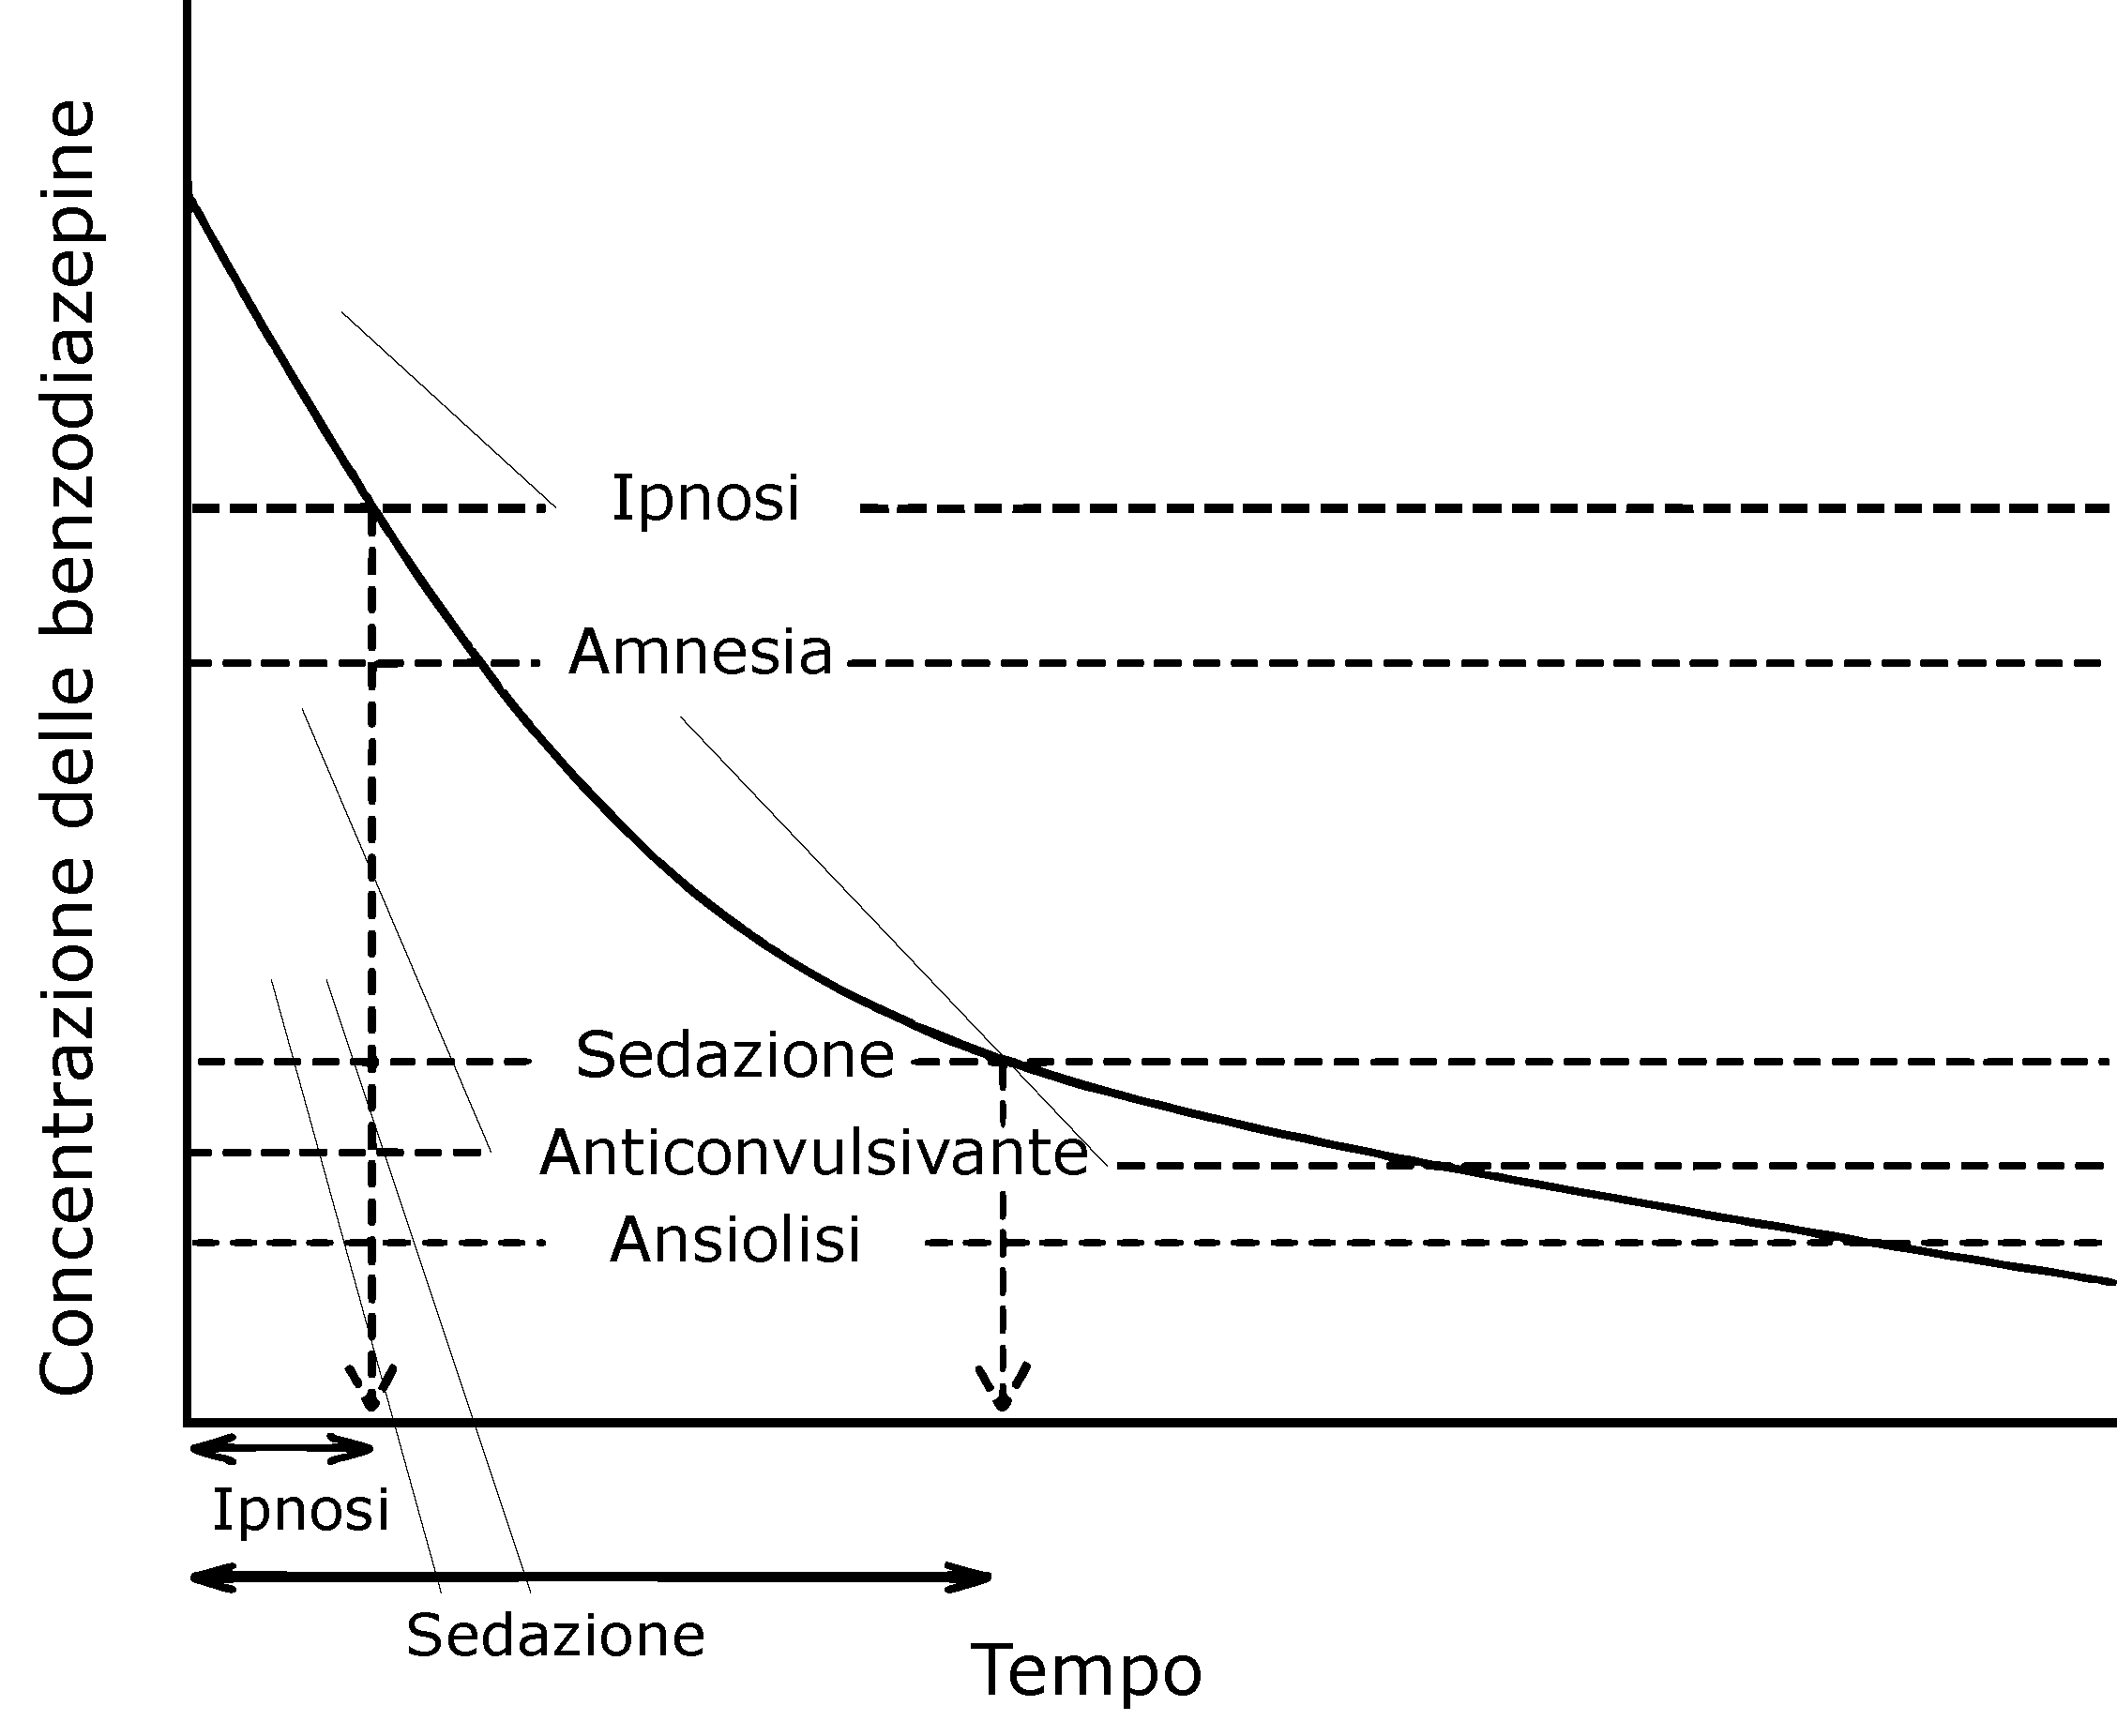
\includegraphics[width=0.7\textwidth]{Figure/figurabenzo.pdf}
    \caption{Relazione tra la concentrazione ematica delle benzodiazepine e i diversi effetti clinici ottenibili, immagine adattata da \cite{Olkkola2008}.}
    \label{fig:benzo}
\end{figure}

\subsection{Farmacocinetica}

\section{Dexmedetomidina}

\lipsum[4]

\section{Protossido di azoto}

\lipsum[5]
 
\end{appendices}

%>RINGRAZIAMENTI
\chapter*{Ringraziamenti}
\addcontentsline{toc}{chapter}{Ringraziamenti}

\lipsum[1-3]

%>BIBLIOGRAFIA
\printbibliography[heading=bibintoc,title={Bibliografia}]

\end{document}

